% lecture6.tex -- GENERATED by build_L6.py from L6_numbers.json; do not edit by hand.
\documentclass[10pt,aspectratio=169,t]{beamer}
% =============================================================================
% emqa_preamble.tex -- shared Beamer preamble of Energy Markets Quantitative Analysis (EMQA)
% Used by every lecture: lectures/Lk/lecturek.tex does
%   \documentclass[10pt,aspectratio=169,t]{beamer}
%   % =============================================================================
% emqa_preamble.tex -- shared Beamer preamble of Energy Markets Quantitative Analysis (EMQA)
% Used by every lecture: lectures/Lk/lecturek.tex does
%   \documentclass[10pt,aspectratio=169,t]{beamer}
%   % =============================================================================
% emqa_preamble.tex -- shared Beamer preamble of Energy Markets Quantitative Analysis (EMQA)
% Used by every lecture: lectures/Lk/lecturek.tex does
%   \documentclass[10pt,aspectratio=169,t]{beamer}
%   \input{../common/emqa_preamble}
%   \emqalecture{k}{Lecture title}
% Logos live in lectures/common/logos/, charts in lectures/Lk/charts/.
% Do NOT add \hfuzz / \vfuzz / \hbadness here: overfull boxes must be fixed, not hidden.
% =============================================================================

\usetheme{default}
\setbeamersize{text margin left=7mm, text margin right=7mm}

% ---------------------------------------------------------------- packages
\usepackage[utf8]{inputenc}
\usepackage[T1]{fontenc}
\usepackage{lmodern}
\usepackage{amsmath, amssymb}
\usepackage{mathtools}
\usepackage{bm}
\usepackage{tikz}
\usetikzlibrary{arrows.meta, positioning, calc, shapes.misc}
\usepackage{booktabs}
\usepackage{array}
\usepackage{graphicx}
\usepackage{colortbl}
\usepackage{xcolor}
\usepackage{multicol}
\hypersetup{colorlinks=true, linkcolor=MainBlue, urlcolor=MainBlue, citecolor=MainBlue}
\graphicspath{{../common/logos/}}   % charts are included with their language folder: charts/en/, charts/ro/

% ---------------------------------------------------------------- colours
\definecolor{MainBlue}{RGB}{26, 58, 110}
\definecolor{IDAred}{RGB}{205, 0, 0}
\definecolor{DarkGray}{RGB}{51, 51, 51}
\definecolor{FooterGray}{RGB}{100, 100, 100}
\definecolor{BlockGray}{RGB}{236, 238, 242}
\definecolor{KeynoteGray}{RGB}{218, 218, 218}
\definecolor{Crimson}{RGB}{190, 40, 50}
\definecolor{Forest}{RGB}{30, 110, 50}
\definecolor{Bitter}{RGB}{214, 150, 20}
% chart palette (same hex values as lectures/common/emqa_plot.py)
\definecolor{SerRO}{HTML}{2A78D6}
\definecolor{SerDE}{HTML}{EB6834}
\definecolor{SerHU}{HTML}{1BAF7A}
\definecolor{SerBG}{HTML}{EDA100}

\setbeamertemplate{background}{%
  \begin{tikzpicture}[remember picture, overlay]
    \shade[shading=axis, shading angle=315, top color=white, bottom color=KeynoteGray]
      (current page.south west) rectangle (current page.north east);
  \end{tikzpicture}}
\setbeamercolor{background canvas}{bg=}
\setbeamercolor{structure}{fg=MainBlue}
\setbeamercolor{normal text}{fg=DarkGray}
\setbeamercolor{title}{fg=IDAred}
\setbeamercolor{frametitle}{fg=IDAred, bg=}
\setbeamercolor{block title}{bg=MainBlue, fg=white}
\setbeamercolor{block body}{bg=BlockGray, fg=DarkGray}
\setbeamercolor{block title alerted}{bg=Crimson, fg=white}
\setbeamercolor{block body alerted}{bg=Crimson!7, fg=DarkGray}
\setbeamercolor{block title example}{bg=Forest, fg=white}
\setbeamercolor{block body example}{bg=Forest!7, fg=DarkGray}
\setbeamercolor{item}{fg=MainBlue}
\setbeamerfont{frametitle}{size=\large, series=\bfseries}
\setbeamerfont{block title}{size=\small, series=\bfseries}
\setbeamertemplate{blocks}[rounded][shadow=false]
\setbeamertemplate{itemize item}{\color{MainBlue}$\boxdot$}
\setbeamertemplate{itemize subitem}{\color{MainBlue}\scriptsize$\blacktriangleright$}
% compact two-level lists: level 1 = main point, level 2 = details (no text outside bullets)
\setbeamerfont{itemize/enumerate subbody}{size=\footnotesize}
\setlength{\leftmargini}{1.1em}
\setlength{\leftmarginii}{1.1em}
\setbeamertemplate{itemize/enumerate body begin}{\setlength{\topsep}{0pt}\setlength{\partopsep}{0pt}\setlength{\parskip}{0pt}}
\setbeamertemplate{itemize/enumerate subbody begin}{\setlength{\topsep}{0pt}\setlength{\partopsep}{0pt}\setlength{\itemsep}{0pt}\vspace{-0.4ex}}

\setbeamertemplate{enumerate item}{\color{MainBlue}\insertenumlabel.}
\setlength{\leftmargini}{1.3em}
\setlength{\leftmarginii}{1.2em}
\setbeamertemplate{navigation symbols}{}
\setbeamertemplate{section in toc}{\color{MainBlue}$\blacktriangleright$~\inserttocsection}
\setbeamertemplate{caption}{\raggedright\insertcaption\par}
% frame subtitle = precise citation line under the claim title (Weron style)
\setbeamerfont{framesubtitle}{size=\footnotesize}
\setbeamercolor{framesubtitle}{fg=FooterGray}
% outline that reappears at every section with the current section highlighted
\setbeamertemplate{section in toc shaded}[default][35]
\setbeamertemplate{subsection in toc shaded}[default][35]
\setbeamertemplate{subsection in toc}{\leavevmode\leftskip=2.2em\color{DarkGray}\small\inserttocsubsection\par}
\AtBeginSection[]{{\begin{frame}{\txtoutline}\vspace{2mm}\small
  \tableofcontents[currentsection,hideothersubsections]\end{frame}}}

% ---------------------------------------------------------------- head and foot
\setbeamertemplate{headline}{%
  \vskip10pt%
  \hbox to \paperwidth{\hskip0.5cm%
    {\small\color{FooterGray}\renewcommand{\hyperlink}[2]{##2}\insertsectionhead}%
    \hfill\textcolor{FooterGray}{\small\insertframenumber}\hskip0.5cm}%
  \vskip4pt{\color{FooterGray}\hrule height 0.4pt}}
% footer as in the other courses (MFM, SFM): course name on the left, small sparkline on the right
\setbeamertemplate{footline}{%
  {\color{FooterGray}\hrule height 0.4pt}\vskip4pt%
  \hbox to \paperwidth{\hskip0.5cm%
    \textcolor{FooterGray}{\small\txtcourse}%
    \hfill\raisebox{-0.1em}{\begin{tikzpicture}[x=0.08em, y=0.08em, line width=0.4pt]
      \draw[FooterGray] (0,3) -- (1,4) -- (2,3.5) -- (3,5) -- (4,4) -- (5,6) -- (6,5.5) -- (7,4) -- (8,5) -- (9,7) -- (10,6) -- (11,5) -- (12,6.5) -- (13,8) -- (14,7) -- (15,6) -- (16,7.5) -- (17,9) -- (18,8) -- (19,7) -- (20,8.5) -- (21,10) -- (22,9) -- (23,8) -- (24,9.5);
    \end{tikzpicture}}\hskip0.5cm}%
  \vskip6pt}

% ---------------------------------------------------------------- title page
\defbeamertemplate*{title page}{emqa}[1][]{%
  \vspace{0.15cm}
  \begin{center}
    \href{https://www.ase.ro}{
\includegraphics[height=0.9cm]{ase_logo.png}}\hspace{0.3cm}%
    \href{https://ipe.ro/new}{
\includegraphics[height=0.9cm]{acad_logo.png}}\hspace{0.3cm}%
    \href{https://theida.net}{
\includegraphics[height=0.9cm]{ida_logo.png}}\hspace{0.3cm}%
    \href{https://blockchain-research-center.com}{
\includegraphics[height=0.9cm]{brc_logo.png}}\hspace{0.3cm}%
    \href{https://www.ai4efin.ase.ro}{
\includegraphics[height=0.9cm]{ai4efin_logo.png}}\hspace{0.3cm}%
    \href{https://www.digital-finance-msca.com}{
\includegraphics[height=0.9cm]{msca_logo.png}}%
  \end{center}
  \vspace{0.45cm}
  \begin{center}
    \begin{minipage}{0.1\textwidth}\centering
      \href{https://quantlet.com}{
\includegraphics[height=0.9cm]{ql_logo.png}}\end{minipage}%
    \begin{minipage}{0.78\textwidth}\centering
      {\Large\bfseries\usebeamercolor[fg]{title}\inserttitle}\par\vspace{0.25cm}
      {\large\usebeamercolor[fg]{title}\insertsubtitle}\end{minipage}%
    \begin{minipage}{0.1\textwidth}\centering
      \href{https://quantinar.com}{
\includegraphics[height=0.9cm]{qr_logo.png}}\end{minipage}
  \end{center}
  \vfill
  \hspace{0.4cm}{\bfseries\insertauthor}\par\vspace{0.12cm}
  \hspace{0.4cm}\begin{minipage}[t]{0.92\textwidth}\raggedright\footnotesize\insertinstitute\end{minipage}
  \par\vspace{0.4cm}}

% ---------------------------------------------------------------- lecture metadata
\newcommand{\emqashort}{}
\newcommand{\emqanb}{notebooks}
\newcommand{\emqarepo}{https://github.com/danpele/EMQA/tree/main}
% language-dependent labels (English default; \emqaromanian switches to Romanian, call it before \emqalecture)
\newcommand{\txtcourse}{Energy Markets Quantitative Analysis}
\newcommand{\txtlecture}{Lecture}
\newcommand{\txtoutline}{Outline}
\newcommand{\txtintuition}{In one sentence:}
\newcommand{\txtjob}{In practice:}
\newcommand{\txttry}{Experiment yourself:}
\newcommand{\txtwhere}{where}
\newcommand{\txtsim}{SIMULATED DATA (teaching illustration)}
\newcommand{\txtnbsuffix}{}
\newcommand{\txtinstitute}{Bucharest University of Economic Studies, Department of Statistics and Econometrics\\
    Romanian Academy, Institute for Economic Forecasting\\
    IDA Institute Digital Assets \textbullet\ AI4EFin \textbullet\ MSCA Digital Finance}
\newcommand{\emqaromanian}{%
  \renewcommand{\txtcourse}{Analiza cantitativă a piețelor de energie}%
  \renewcommand{\txtlecture}{Cursul}%
  \renewcommand{\txtoutline}{Cuprins}%
  \renewcommand{\txtintuition}{Pe scurt:}%
  \renewcommand{\txtjob}{În practică:}%
  \renewcommand{\txttry}{Exercițiu practic:}%
  \renewcommand{\txtwhere}{unde}%
  \renewcommand{\txtsim}{DATE SIMULATE (doar pentru ilustrare)}%
  \renewcommand{\txtnbsuffix}{\string_ro}%
  \renewcommand{\txtinstitute}{Academia de Studii Economice din București, Departamentul de Statistică și Econometrie\\
    Academia Română, Institutul de Prognoză Economică\\
    IDA Institute Digital Assets \textbullet\ AI4EFin \textbullet\ MSCA Digital Finance}}
\newcommand{\emqalecture}[2]{%
  \renewcommand{\emqashort}{\txtlecture\ #1}%
  \renewcommand{\emqanb}{notebooks/L#1\string_notebook\txtnbsuffix.ipynb}%
  \title[EMQA]{\txtcourse}%
  \subtitle{\txtlecture\ #1: #2}%
  \author{Prof.\ dr.\ Daniel Traian PELE}%
  \institute{\txtinstitute}%
  \date{}}

% ---------------------------------------------------------------- teaching blocks (MBA clarity rule)
% \intuition{one plain sentence}  ->  formula with every symbol defined  ->  real-data example  ->  \manager{one line}
\newcommand{\intuition}[1]{\begin{itemize}\item {\color{MainBlue}\textbf{\txtintuition}}~#1\end{itemize}\vspace{0.6mm}}
\newcommand{\manager}[1]{\colorbox{Forest!10}{\parbox{\dimexpr\linewidth-2\fboxsep\relax}{\footnotesize
  \begin{itemize}\setlength{\itemsep}{0pt}\item \textbf{\color{Forest}\txtjob}~#1\end{itemize}}}}
% Experiment yourself: pointer to the matching notebook section
\newcommand{\tryit}[1]{{\scriptsize\href{\emqarepo/\emqanb}{%
  \raisebox{-0.15em}{
\includegraphics[height=0.85em]{ql_logo.png}}\,\textbf{\txttry}~\color{MainBlue}#1}}}
% bottom row: manager line (left) + experiment pointer (right), pinned to the bottom of the frame
\newcommand{\bottomrow}[2]{\par\vfill\noindent\begin{minipage}[b]{0.72\linewidth}#1\end{minipage}\hfill
  \begin{minipage}[b]{0.26\linewidth}\raggedleft #2\end{minipage}\par\vspace{0.5mm}}
\newcommand{\where}[1]{{\footnotesize\textbf{\txtwhere}~#1\par}}

% ---------------------------------------------------------------- helpers
% chart source line under a figure: \chartsource{Source ...; period ...}
\newcommand{\chartsource}[1]{\par\vspace{1pt}{\scriptsize\color{FooterGray}#1\par}}
% link to code: \quantlet{label}{path inside the repo}
\newcommand{\quantlet}[2]{\par\vspace{1pt}\hfill\href{\emqarepo/#2}{%
  \raisebox{-0.15em}{
\includegraphics[height=0.75em]{ql_logo.png}}\textcolor{MainBlue}{\scriptsize\ #1}}}
\newcommand{\simlabel}{\colorbox{Crimson!12}{\scriptsize\bfseries\color{Crimson}\txtsim}}
\newcommand{\E}{\mathbb{E}}
\newcommand{\Var}{\operatorname{Var}}
\newcommand{\Cov}{\operatorname{Cov}}
\newcommand{\Corr}{\operatorname{Corr}}
\newcommand{\asinh}{\operatorname{asinh}}
\newcommand{\iid}{\overset{\text{i.i.d.}}{\sim}}
\newcommand{\EUR}{EUR}

%   \emqalecture{k}{Lecture title}
% Logos live in lectures/common/logos/, charts in lectures/Lk/charts/.
% Do NOT add \hfuzz / \vfuzz / \hbadness here: overfull boxes must be fixed, not hidden.
% =============================================================================

\usetheme{default}
\setbeamersize{text margin left=7mm, text margin right=7mm}

% ---------------------------------------------------------------- packages
\usepackage[utf8]{inputenc}
\usepackage[T1]{fontenc}
\usepackage{lmodern}
\usepackage{amsmath, amssymb}
\usepackage{mathtools}
\usepackage{bm}
\usepackage{tikz}
\usetikzlibrary{arrows.meta, positioning, calc, shapes.misc}
\usepackage{booktabs}
\usepackage{array}
\usepackage{graphicx}
\usepackage{colortbl}
\usepackage{xcolor}
\usepackage{multicol}
\hypersetup{colorlinks=true, linkcolor=MainBlue, urlcolor=MainBlue, citecolor=MainBlue}
\graphicspath{{../common/logos/}}   % charts are included with their language folder: charts/en/, charts/ro/

% ---------------------------------------------------------------- colours
\definecolor{MainBlue}{RGB}{26, 58, 110}
\definecolor{IDAred}{RGB}{205, 0, 0}
\definecolor{DarkGray}{RGB}{51, 51, 51}
\definecolor{FooterGray}{RGB}{100, 100, 100}
\definecolor{BlockGray}{RGB}{236, 238, 242}
\definecolor{KeynoteGray}{RGB}{218, 218, 218}
\definecolor{Crimson}{RGB}{190, 40, 50}
\definecolor{Forest}{RGB}{30, 110, 50}
\definecolor{Bitter}{RGB}{214, 150, 20}
% chart palette (same hex values as lectures/common/emqa_plot.py)
\definecolor{SerRO}{HTML}{2A78D6}
\definecolor{SerDE}{HTML}{EB6834}
\definecolor{SerHU}{HTML}{1BAF7A}
\definecolor{SerBG}{HTML}{EDA100}

\setbeamertemplate{background}{%
  \begin{tikzpicture}[remember picture, overlay]
    \shade[shading=axis, shading angle=315, top color=white, bottom color=KeynoteGray]
      (current page.south west) rectangle (current page.north east);
  \end{tikzpicture}}
\setbeamercolor{background canvas}{bg=}
\setbeamercolor{structure}{fg=MainBlue}
\setbeamercolor{normal text}{fg=DarkGray}
\setbeamercolor{title}{fg=IDAred}
\setbeamercolor{frametitle}{fg=IDAred, bg=}
\setbeamercolor{block title}{bg=MainBlue, fg=white}
\setbeamercolor{block body}{bg=BlockGray, fg=DarkGray}
\setbeamercolor{block title alerted}{bg=Crimson, fg=white}
\setbeamercolor{block body alerted}{bg=Crimson!7, fg=DarkGray}
\setbeamercolor{block title example}{bg=Forest, fg=white}
\setbeamercolor{block body example}{bg=Forest!7, fg=DarkGray}
\setbeamercolor{item}{fg=MainBlue}
\setbeamerfont{frametitle}{size=\large, series=\bfseries}
\setbeamerfont{block title}{size=\small, series=\bfseries}
\setbeamertemplate{blocks}[rounded][shadow=false]
\setbeamertemplate{itemize item}{\color{MainBlue}$\boxdot$}
\setbeamertemplate{itemize subitem}{\color{MainBlue}\scriptsize$\blacktriangleright$}
% compact two-level lists: level 1 = main point, level 2 = details (no text outside bullets)
\setbeamerfont{itemize/enumerate subbody}{size=\footnotesize}
\setlength{\leftmargini}{1.1em}
\setlength{\leftmarginii}{1.1em}
\setbeamertemplate{itemize/enumerate body begin}{\setlength{\topsep}{0pt}\setlength{\partopsep}{0pt}\setlength{\parskip}{0pt}}
\setbeamertemplate{itemize/enumerate subbody begin}{\setlength{\topsep}{0pt}\setlength{\partopsep}{0pt}\setlength{\itemsep}{0pt}\vspace{-0.4ex}}

\setbeamertemplate{enumerate item}{\color{MainBlue}\insertenumlabel.}
\setlength{\leftmargini}{1.3em}
\setlength{\leftmarginii}{1.2em}
\setbeamertemplate{navigation symbols}{}
\setbeamertemplate{section in toc}{\color{MainBlue}$\blacktriangleright$~\inserttocsection}
\setbeamertemplate{caption}{\raggedright\insertcaption\par}
% frame subtitle = precise citation line under the claim title (Weron style)
\setbeamerfont{framesubtitle}{size=\footnotesize}
\setbeamercolor{framesubtitle}{fg=FooterGray}
% outline that reappears at every section with the current section highlighted
\setbeamertemplate{section in toc shaded}[default][35]
\setbeamertemplate{subsection in toc shaded}[default][35]
\setbeamertemplate{subsection in toc}{\leavevmode\leftskip=2.2em\color{DarkGray}\small\inserttocsubsection\par}
\AtBeginSection[]{{\begin{frame}{\txtoutline}\vspace{2mm}\small
  \tableofcontents[currentsection,hideothersubsections]\end{frame}}}

% ---------------------------------------------------------------- head and foot
\setbeamertemplate{headline}{%
  \vskip10pt%
  \hbox to \paperwidth{\hskip0.5cm%
    {\small\color{FooterGray}\renewcommand{\hyperlink}[2]{##2}\insertsectionhead}%
    \hfill\textcolor{FooterGray}{\small\insertframenumber}\hskip0.5cm}%
  \vskip4pt{\color{FooterGray}\hrule height 0.4pt}}
% footer as in the other courses (MFM, SFM): course name on the left, small sparkline on the right
\setbeamertemplate{footline}{%
  {\color{FooterGray}\hrule height 0.4pt}\vskip4pt%
  \hbox to \paperwidth{\hskip0.5cm%
    \textcolor{FooterGray}{\small\txtcourse}%
    \hfill\raisebox{-0.1em}{\begin{tikzpicture}[x=0.08em, y=0.08em, line width=0.4pt]
      \draw[FooterGray] (0,3) -- (1,4) -- (2,3.5) -- (3,5) -- (4,4) -- (5,6) -- (6,5.5) -- (7,4) -- (8,5) -- (9,7) -- (10,6) -- (11,5) -- (12,6.5) -- (13,8) -- (14,7) -- (15,6) -- (16,7.5) -- (17,9) -- (18,8) -- (19,7) -- (20,8.5) -- (21,10) -- (22,9) -- (23,8) -- (24,9.5);
    \end{tikzpicture}}\hskip0.5cm}%
  \vskip6pt}

% ---------------------------------------------------------------- title page
\defbeamertemplate*{title page}{emqa}[1][]{%
  \vspace{0.15cm}
  \begin{center}
    \href{https://www.ase.ro}{
\includegraphics[height=0.9cm]{ase_logo.png}}\hspace{0.3cm}%
    \href{https://ipe.ro/new}{
\includegraphics[height=0.9cm]{acad_logo.png}}\hspace{0.3cm}%
    \href{https://theida.net}{
\includegraphics[height=0.9cm]{ida_logo.png}}\hspace{0.3cm}%
    \href{https://blockchain-research-center.com}{
\includegraphics[height=0.9cm]{brc_logo.png}}\hspace{0.3cm}%
    \href{https://www.ai4efin.ase.ro}{
\includegraphics[height=0.9cm]{ai4efin_logo.png}}\hspace{0.3cm}%
    \href{https://www.digital-finance-msca.com}{
\includegraphics[height=0.9cm]{msca_logo.png}}%
  \end{center}
  \vspace{0.45cm}
  \begin{center}
    \begin{minipage}{0.1\textwidth}\centering
      \href{https://quantlet.com}{
\includegraphics[height=0.9cm]{ql_logo.png}}\end{minipage}%
    \begin{minipage}{0.78\textwidth}\centering
      {\Large\bfseries\usebeamercolor[fg]{title}\inserttitle}\par\vspace{0.25cm}
      {\large\usebeamercolor[fg]{title}\insertsubtitle}\end{minipage}%
    \begin{minipage}{0.1\textwidth}\centering
      \href{https://quantinar.com}{
\includegraphics[height=0.9cm]{qr_logo.png}}\end{minipage}
  \end{center}
  \vfill
  \hspace{0.4cm}{\bfseries\insertauthor}\par\vspace{0.12cm}
  \hspace{0.4cm}\begin{minipage}[t]{0.92\textwidth}\raggedright\footnotesize\insertinstitute\end{minipage}
  \par\vspace{0.4cm}}

% ---------------------------------------------------------------- lecture metadata
\newcommand{\emqashort}{}
\newcommand{\emqanb}{notebooks}
\newcommand{\emqarepo}{https://github.com/danpele/EMQA/tree/main}
% language-dependent labels (English default; \emqaromanian switches to Romanian, call it before \emqalecture)
\newcommand{\txtcourse}{Energy Markets Quantitative Analysis}
\newcommand{\txtlecture}{Lecture}
\newcommand{\txtoutline}{Outline}
\newcommand{\txtintuition}{In one sentence:}
\newcommand{\txtjob}{In practice:}
\newcommand{\txttry}{Experiment yourself:}
\newcommand{\txtwhere}{where}
\newcommand{\txtsim}{SIMULATED DATA (teaching illustration)}
\newcommand{\txtnbsuffix}{}
\newcommand{\txtinstitute}{Bucharest University of Economic Studies, Department of Statistics and Econometrics\\
    Romanian Academy, Institute for Economic Forecasting\\
    IDA Institute Digital Assets \textbullet\ AI4EFin \textbullet\ MSCA Digital Finance}
\newcommand{\emqaromanian}{%
  \renewcommand{\txtcourse}{Analiza cantitativă a piețelor de energie}%
  \renewcommand{\txtlecture}{Cursul}%
  \renewcommand{\txtoutline}{Cuprins}%
  \renewcommand{\txtintuition}{Pe scurt:}%
  \renewcommand{\txtjob}{În practică:}%
  \renewcommand{\txttry}{Exercițiu practic:}%
  \renewcommand{\txtwhere}{unde}%
  \renewcommand{\txtsim}{DATE SIMULATE (doar pentru ilustrare)}%
  \renewcommand{\txtnbsuffix}{\string_ro}%
  \renewcommand{\txtinstitute}{Academia de Studii Economice din București, Departamentul de Statistică și Econometrie\\
    Academia Română, Institutul de Prognoză Economică\\
    IDA Institute Digital Assets \textbullet\ AI4EFin \textbullet\ MSCA Digital Finance}}
\newcommand{\emqalecture}[2]{%
  \renewcommand{\emqashort}{\txtlecture\ #1}%
  \renewcommand{\emqanb}{notebooks/L#1\string_notebook\txtnbsuffix.ipynb}%
  \title[EMQA]{\txtcourse}%
  \subtitle{\txtlecture\ #1: #2}%
  \author{Prof.\ dr.\ Daniel Traian PELE}%
  \institute{\txtinstitute}%
  \date{}}

% ---------------------------------------------------------------- teaching blocks (MBA clarity rule)
% \intuition{one plain sentence}  ->  formula with every symbol defined  ->  real-data example  ->  \manager{one line}
\newcommand{\intuition}[1]{\begin{itemize}\item {\color{MainBlue}\textbf{\txtintuition}}~#1\end{itemize}\vspace{0.6mm}}
\newcommand{\manager}[1]{\colorbox{Forest!10}{\parbox{\dimexpr\linewidth-2\fboxsep\relax}{\footnotesize
  \begin{itemize}\setlength{\itemsep}{0pt}\item \textbf{\color{Forest}\txtjob}~#1\end{itemize}}}}
% Experiment yourself: pointer to the matching notebook section
\newcommand{\tryit}[1]{{\scriptsize\href{\emqarepo/\emqanb}{%
  \raisebox{-0.15em}{
\includegraphics[height=0.85em]{ql_logo.png}}\,\textbf{\txttry}~\color{MainBlue}#1}}}
% bottom row: manager line (left) + experiment pointer (right), pinned to the bottom of the frame
\newcommand{\bottomrow}[2]{\par\vfill\noindent\begin{minipage}[b]{0.72\linewidth}#1\end{minipage}\hfill
  \begin{minipage}[b]{0.26\linewidth}\raggedleft #2\end{minipage}\par\vspace{0.5mm}}
\newcommand{\where}[1]{{\footnotesize\textbf{\txtwhere}~#1\par}}

% ---------------------------------------------------------------- helpers
% chart source line under a figure: \chartsource{Source ...; period ...}
\newcommand{\chartsource}[1]{\par\vspace{1pt}{\scriptsize\color{FooterGray}#1\par}}
% link to code: \quantlet{label}{path inside the repo}
\newcommand{\quantlet}[2]{\par\vspace{1pt}\hfill\href{\emqarepo/#2}{%
  \raisebox{-0.15em}{
\includegraphics[height=0.75em]{ql_logo.png}}\textcolor{MainBlue}{\scriptsize\ #1}}}
\newcommand{\simlabel}{\colorbox{Crimson!12}{\scriptsize\bfseries\color{Crimson}\txtsim}}
\newcommand{\E}{\mathbb{E}}
\newcommand{\Var}{\operatorname{Var}}
\newcommand{\Cov}{\operatorname{Cov}}
\newcommand{\Corr}{\operatorname{Corr}}
\newcommand{\asinh}{\operatorname{asinh}}
\newcommand{\iid}{\overset{\text{i.i.d.}}{\sim}}
\newcommand{\EUR}{EUR}

%   \emqalecture{k}{Lecture title}
% Logos live in lectures/common/logos/, charts in lectures/Lk/charts/.
% Do NOT add \hfuzz / \vfuzz / \hbadness here: overfull boxes must be fixed, not hidden.
% =============================================================================

\usetheme{default}
\setbeamersize{text margin left=7mm, text margin right=7mm}

% ---------------------------------------------------------------- packages
\usepackage[utf8]{inputenc}
\usepackage[T1]{fontenc}
\usepackage{lmodern}
\usepackage{amsmath, amssymb}
\usepackage{mathtools}
\usepackage{bm}
\usepackage{tikz}
\usetikzlibrary{arrows.meta, positioning, calc, shapes.misc}
\usepackage{booktabs}
\usepackage{array}
\usepackage{graphicx}
\usepackage{colortbl}
\usepackage{xcolor}
\usepackage{multicol}
\hypersetup{colorlinks=true, linkcolor=MainBlue, urlcolor=MainBlue, citecolor=MainBlue}
\graphicspath{{../common/logos/}}   % charts are included with their language folder: charts/en/, charts/ro/

% ---------------------------------------------------------------- colours
\definecolor{MainBlue}{RGB}{26, 58, 110}
\definecolor{IDAred}{RGB}{205, 0, 0}
\definecolor{DarkGray}{RGB}{51, 51, 51}
\definecolor{FooterGray}{RGB}{100, 100, 100}
\definecolor{BlockGray}{RGB}{236, 238, 242}
\definecolor{KeynoteGray}{RGB}{218, 218, 218}
\definecolor{Crimson}{RGB}{190, 40, 50}
\definecolor{Forest}{RGB}{30, 110, 50}
\definecolor{Bitter}{RGB}{214, 150, 20}
% chart palette (same hex values as lectures/common/emqa_plot.py)
\definecolor{SerRO}{HTML}{2A78D6}
\definecolor{SerDE}{HTML}{EB6834}
\definecolor{SerHU}{HTML}{1BAF7A}
\definecolor{SerBG}{HTML}{EDA100}

\setbeamertemplate{background}{%
  \begin{tikzpicture}[remember picture, overlay]
    \shade[shading=axis, shading angle=315, top color=white, bottom color=KeynoteGray]
      (current page.south west) rectangle (current page.north east);
  \end{tikzpicture}}
\setbeamercolor{background canvas}{bg=}
\setbeamercolor{structure}{fg=MainBlue}
\setbeamercolor{normal text}{fg=DarkGray}
\setbeamercolor{title}{fg=IDAred}
\setbeamercolor{frametitle}{fg=IDAred, bg=}
\setbeamercolor{block title}{bg=MainBlue, fg=white}
\setbeamercolor{block body}{bg=BlockGray, fg=DarkGray}
\setbeamercolor{block title alerted}{bg=Crimson, fg=white}
\setbeamercolor{block body alerted}{bg=Crimson!7, fg=DarkGray}
\setbeamercolor{block title example}{bg=Forest, fg=white}
\setbeamercolor{block body example}{bg=Forest!7, fg=DarkGray}
\setbeamercolor{item}{fg=MainBlue}
\setbeamerfont{frametitle}{size=\large, series=\bfseries}
\setbeamerfont{block title}{size=\small, series=\bfseries}
\setbeamertemplate{blocks}[rounded][shadow=false]
\setbeamertemplate{itemize item}{\color{MainBlue}$\boxdot$}
\setbeamertemplate{itemize subitem}{\color{MainBlue}\scriptsize$\blacktriangleright$}
% compact two-level lists: level 1 = main point, level 2 = details (no text outside bullets)
\setbeamerfont{itemize/enumerate subbody}{size=\footnotesize}
\setlength{\leftmargini}{1.1em}
\setlength{\leftmarginii}{1.1em}
\setbeamertemplate{itemize/enumerate body begin}{\setlength{\topsep}{0pt}\setlength{\partopsep}{0pt}\setlength{\parskip}{0pt}}
\setbeamertemplate{itemize/enumerate subbody begin}{\setlength{\topsep}{0pt}\setlength{\partopsep}{0pt}\setlength{\itemsep}{0pt}\vspace{-0.4ex}}

\setbeamertemplate{enumerate item}{\color{MainBlue}\insertenumlabel.}
\setlength{\leftmargini}{1.3em}
\setlength{\leftmarginii}{1.2em}
\setbeamertemplate{navigation symbols}{}
\setbeamertemplate{section in toc}{\color{MainBlue}$\blacktriangleright$~\inserttocsection}
\setbeamertemplate{caption}{\raggedright\insertcaption\par}
% frame subtitle = precise citation line under the claim title (Weron style)
\setbeamerfont{framesubtitle}{size=\footnotesize}
\setbeamercolor{framesubtitle}{fg=FooterGray}
% outline that reappears at every section with the current section highlighted
\setbeamertemplate{section in toc shaded}[default][35]
\setbeamertemplate{subsection in toc shaded}[default][35]
\setbeamertemplate{subsection in toc}{\leavevmode\leftskip=2.2em\color{DarkGray}\small\inserttocsubsection\par}
\AtBeginSection[]{{\begin{frame}{\txtoutline}\vspace{2mm}\small
  \tableofcontents[currentsection,hideothersubsections]\end{frame}}}

% ---------------------------------------------------------------- head and foot
\setbeamertemplate{headline}{%
  \vskip10pt%
  \hbox to \paperwidth{\hskip0.5cm%
    {\small\color{FooterGray}\renewcommand{\hyperlink}[2]{##2}\insertsectionhead}%
    \hfill\textcolor{FooterGray}{\small\insertframenumber}\hskip0.5cm}%
  \vskip4pt{\color{FooterGray}\hrule height 0.4pt}}
% footer as in the other courses (MFM, SFM): course name on the left, small sparkline on the right
\setbeamertemplate{footline}{%
  {\color{FooterGray}\hrule height 0.4pt}\vskip4pt%
  \hbox to \paperwidth{\hskip0.5cm%
    \textcolor{FooterGray}{\small\txtcourse}%
    \hfill\raisebox{-0.1em}{\begin{tikzpicture}[x=0.08em, y=0.08em, line width=0.4pt]
      \draw[FooterGray] (0,3) -- (1,4) -- (2,3.5) -- (3,5) -- (4,4) -- (5,6) -- (6,5.5) -- (7,4) -- (8,5) -- (9,7) -- (10,6) -- (11,5) -- (12,6.5) -- (13,8) -- (14,7) -- (15,6) -- (16,7.5) -- (17,9) -- (18,8) -- (19,7) -- (20,8.5) -- (21,10) -- (22,9) -- (23,8) -- (24,9.5);
    \end{tikzpicture}}\hskip0.5cm}%
  \vskip6pt}

% ---------------------------------------------------------------- title page
\defbeamertemplate*{title page}{emqa}[1][]{%
  \vspace{0.15cm}
  \begin{center}
    \href{https://www.ase.ro}{
\includegraphics[height=0.9cm]{ase_logo.png}}\hspace{0.3cm}%
    \href{https://ipe.ro/new}{
\includegraphics[height=0.9cm]{acad_logo.png}}\hspace{0.3cm}%
    \href{https://theida.net}{
\includegraphics[height=0.9cm]{ida_logo.png}}\hspace{0.3cm}%
    \href{https://blockchain-research-center.com}{
\includegraphics[height=0.9cm]{brc_logo.png}}\hspace{0.3cm}%
    \href{https://www.ai4efin.ase.ro}{
\includegraphics[height=0.9cm]{ai4efin_logo.png}}\hspace{0.3cm}%
    \href{https://www.digital-finance-msca.com}{
\includegraphics[height=0.9cm]{msca_logo.png}}%
  \end{center}
  \vspace{0.45cm}
  \begin{center}
    \begin{minipage}{0.1\textwidth}\centering
      \href{https://quantlet.com}{
\includegraphics[height=0.9cm]{ql_logo.png}}\end{minipage}%
    \begin{minipage}{0.78\textwidth}\centering
      {\Large\bfseries\usebeamercolor[fg]{title}\inserttitle}\par\vspace{0.25cm}
      {\large\usebeamercolor[fg]{title}\insertsubtitle}\end{minipage}%
    \begin{minipage}{0.1\textwidth}\centering
      \href{https://quantinar.com}{
\includegraphics[height=0.9cm]{qr_logo.png}}\end{minipage}
  \end{center}
  \vfill
  \hspace{0.4cm}{\bfseries\insertauthor}\par\vspace{0.12cm}
  \hspace{0.4cm}\begin{minipage}[t]{0.92\textwidth}\raggedright\footnotesize\insertinstitute\end{minipage}
  \par\vspace{0.4cm}}

% ---------------------------------------------------------------- lecture metadata
\newcommand{\emqashort}{}
\newcommand{\emqanb}{notebooks}
\newcommand{\emqarepo}{https://github.com/danpele/EMQA/tree/main}
% language-dependent labels (English default; \emqaromanian switches to Romanian, call it before \emqalecture)
\newcommand{\txtcourse}{Energy Markets Quantitative Analysis}
\newcommand{\txtlecture}{Lecture}
\newcommand{\txtoutline}{Outline}
\newcommand{\txtintuition}{In one sentence:}
\newcommand{\txtjob}{In practice:}
\newcommand{\txttry}{Experiment yourself:}
\newcommand{\txtwhere}{where}
\newcommand{\txtsim}{SIMULATED DATA (teaching illustration)}
\newcommand{\txtnbsuffix}{}
\newcommand{\txtinstitute}{Bucharest University of Economic Studies, Department of Statistics and Econometrics\\
    Romanian Academy, Institute for Economic Forecasting\\
    IDA Institute Digital Assets \textbullet\ AI4EFin \textbullet\ MSCA Digital Finance}
\newcommand{\emqaromanian}{%
  \renewcommand{\txtcourse}{Analiza cantitativă a piețelor de energie}%
  \renewcommand{\txtlecture}{Cursul}%
  \renewcommand{\txtoutline}{Cuprins}%
  \renewcommand{\txtintuition}{Pe scurt:}%
  \renewcommand{\txtjob}{În practică:}%
  \renewcommand{\txttry}{Exercițiu practic:}%
  \renewcommand{\txtwhere}{unde}%
  \renewcommand{\txtsim}{DATE SIMULATE (doar pentru ilustrare)}%
  \renewcommand{\txtnbsuffix}{\string_ro}%
  \renewcommand{\txtinstitute}{Academia de Studii Economice din București, Departamentul de Statistică și Econometrie\\
    Academia Română, Institutul de Prognoză Economică\\
    IDA Institute Digital Assets \textbullet\ AI4EFin \textbullet\ MSCA Digital Finance}}
\newcommand{\emqalecture}[2]{%
  \renewcommand{\emqashort}{\txtlecture\ #1}%
  \renewcommand{\emqanb}{notebooks/L#1\string_notebook\txtnbsuffix.ipynb}%
  \title[EMQA]{\txtcourse}%
  \subtitle{\txtlecture\ #1: #2}%
  \author{Prof.\ dr.\ Daniel Traian PELE}%
  \institute{\txtinstitute}%
  \date{}}

% ---------------------------------------------------------------- teaching blocks (MBA clarity rule)
% \intuition{one plain sentence}  ->  formula with every symbol defined  ->  real-data example  ->  \manager{one line}
\newcommand{\intuition}[1]{\begin{itemize}\item {\color{MainBlue}\textbf{\txtintuition}}~#1\end{itemize}\vspace{0.6mm}}
\newcommand{\manager}[1]{\colorbox{Forest!10}{\parbox{\dimexpr\linewidth-2\fboxsep\relax}{\footnotesize
  \begin{itemize}\setlength{\itemsep}{0pt}\item \textbf{\color{Forest}\txtjob}~#1\end{itemize}}}}
% Experiment yourself: pointer to the matching notebook section
\newcommand{\tryit}[1]{{\scriptsize\href{\emqarepo/\emqanb}{%
  \raisebox{-0.15em}{
\includegraphics[height=0.85em]{ql_logo.png}}\,\textbf{\txttry}~\color{MainBlue}#1}}}
% bottom row: manager line (left) + experiment pointer (right), pinned to the bottom of the frame
\newcommand{\bottomrow}[2]{\par\vfill\noindent\begin{minipage}[b]{0.72\linewidth}#1\end{minipage}\hfill
  \begin{minipage}[b]{0.26\linewidth}\raggedleft #2\end{minipage}\par\vspace{0.5mm}}
\newcommand{\where}[1]{{\footnotesize\textbf{\txtwhere}~#1\par}}

% ---------------------------------------------------------------- helpers
% chart source line under a figure: \chartsource{Source ...; period ...}
\newcommand{\chartsource}[1]{\par\vspace{1pt}{\scriptsize\color{FooterGray}#1\par}}
% link to code: \quantlet{label}{path inside the repo}
\newcommand{\quantlet}[2]{\par\vspace{1pt}\hfill\href{\emqarepo/#2}{%
  \raisebox{-0.15em}{
\includegraphics[height=0.75em]{ql_logo.png}}\textcolor{MainBlue}{\scriptsize\ #1}}}
\newcommand{\simlabel}{\colorbox{Crimson!12}{\scriptsize\bfseries\color{Crimson}\txtsim}}
\newcommand{\E}{\mathbb{E}}
\newcommand{\Var}{\operatorname{Var}}
\newcommand{\Cov}{\operatorname{Cov}}
\newcommand{\Corr}{\operatorname{Corr}}
\newcommand{\asinh}{\operatorname{asinh}}
\newcommand{\iid}{\overset{\text{i.i.d.}}{\sim}}
\newcommand{\EUR}{EUR}

\emqalecture{6}{Renewables and Storage: Cannibalisation, Negative Prices and Batteries}
\begin{document}
{\setbeamertemplate{headline}{}\setbeamertemplate{footline}{}
\begin{frame}\titlepage\end{frame}}
% END-FRONT-MATTER

\begin{frame}{Learning objectives}
\small
\begin{itemize}\setlength{\itemsep}{3pt}
  \item \textbf{Merit order}
    \begin{itemize}\setlength{\itemsep}{0pt}
      \item Measure how much zero-cost solar and wind lower the price of the Romanian day-ahead market (PZU)
      \item On the real order book and with a regression on hourly data
    \end{itemize}
  \item \textbf{Capture price and capture rate}
    \begin{itemize}\setlength{\itemsep}{0pt}
      \item The price a solar or wind MWh actually earns, compared with the average price
      \item Cannibalisation: the more solar, the lower its own price
    \end{itemize}
  \item \textbf{Negative prices and the daily price shape}
    \begin{itemize}\setlength{\itemsep}{0pt}
      \item Count negative prices in hour-equivalents; value switching a park off
      \item Read the 15-minute daily profile
    \end{itemize}
  \item \textbf{Batteries}
    \begin{itemize}\setlength{\itemsep}{0pt}
      \item Arbitrage revenue of 1-, 2- and 4-hour batteries from a linear programme (LP)
      \item Perfect foresight vs forecast rules, hourly vs 15-minute prices, Romania vs neighbours
    \end{itemize}
\end{itemize}
\end{frame}

% BEGIN-ABBR

\begin{frame}{Abbreviations}
\small
\vspace{-1mm}\begin{columns}[T,onlytextwidth]
\begin{column}{0.49\textwidth}{\scriptsize\renewcommand{\arraystretch}{1.0}\begin{tabular}{@{}>{\bfseries}l@{\ \ }p{0.76\linewidth}@{}}AI & artificial intelligence\\
BG & Bulgaria (bidding zone)\\
CET & Central European Time\\
CP & capture price\\
CR & capture rate (value factor)\\
DE-LU & Germany--Luxembourg bidding zone\\
ENTSO-E & European Network of Transmission System Operators for Electricity\\
EPEX & EPEX SPOT power exchange\\
EUR & euro\\
GW & gigawatt = 1\,000 MW\\
HAC & heteroskedasticity- and autocorrelation-consistent (standard errors)\\
HU & Hungary (bidding zone)\\
HUPX & Hungarian Power Exchange\\
IBEX & Independent Bulgarian Energy Exchange\\
ISE & Fraunhofer Institute for Solar Energy Systems\\
kW & kilowatt\\\end{tabular}}\end{column}
\begin{column}{0.49\textwidth}{\scriptsize\renewcommand{\arraystretch}{1.0}\begin{tabular}{@{}>{\bfseries}l@{\ \ }p{0.76\linewidth}@{}}kWh & kilowatt-hour\\
LP & linear programme\\
MTU & market time unit\\
MW & megawatt\\
MWh & megawatt-hour\\
NREL & National Renewable Energy Laboratory (United States)\\
OLS & ordinary least squares\\
OPCOM & Romanian electricity and gas market operator\\
PPA & power purchase agreement\\
PZU & Piața pentru Ziua Următoare (day-ahead market)\\
RO & Romania (bidding zone)\\
SDAC & Single Day-Ahead Coupling\\
SE & standard error\\
TWh & terawatt-hour\\
XML & Extensible Markup Language (data file format)\\\end{tabular}}\end{column}
\end{columns}
\end{frame}

% END-ABBR

\begin{frame}{Real data only: prices, generation, order books, installed capacity}
\footnotesize
{\scriptsize\renewcommand{\arraystretch}{0.95}\setlength{\tabcolsep}{4pt}
\begin{tabular}{@{}p{0.30\textwidth}p{0.15\textwidth}p{0.50\textwidth}@{}}\toprule
Series & Frequency & Source \\ \midrule
Day-ahead prices: Romania (RO), Bulgaria (BG), Hungary (HU), Germany--Luxembourg (DE-LU) & hourly; 15-min from 1 Oct 2025 & Romanian market operator (OPCOM), Independent Bulgarian Energy Exchange (IBEX), Hungarian Power Exchange (HUPX), European Power Exchange (EPEX SPOT); via energy-charts.info (Fraunhofer ISE) \\
Solar, wind, battery output, load & RO, HU 15-min; BG hourly & European Network of Transmission System Operators for Electricity (ENTSO-E); Transelectrica data for RO \\
PZU supply and demand curves & 2 quarter-hours & OPCOM, Extensible Markup Language (XML) files \\
Installed capacity & yearly & ENTSO-E via energy-charts.info \\
\bottomrule\end{tabular}}
\vspace{1mm}
\begin{itemize}\setlength{\itemsep}{1pt}
  \item \textbf{Period}: 2019 -- 31 Oct 2026, the last complete month
    \begin{itemize}\setlength{\itemsep}{0pt}
      \item 2026 = Jan--Oct 2026; ``last 12 months'' = Nov 2025 -- Oct 2026
      \item Delivery days in Central European Time (CET)
    \end{itemize}
  \item \textbf{Conventions}
    \begin{itemize}\setlength{\itemsep}{0pt}
      \item Energy = mean MW $\times$ duration; a 15-minute market time unit (MTU) counts 0.25 h
    \end{itemize}
\end{itemize}
\par\vfill\noindent{\scriptsize\color{FooterGray}(data/SOURCES.md; data/download\_L6.py)}\hfill\tryit{notebook \S1}\par\vspace{0.5mm}
\end{frame}


\section{Renewables and the merit order}

\subsection{The solar boom}

\begin{frame}{Installed solar in Romania grew 2.4 times from 2019 to 2025}
\footnotesize
\begin{center}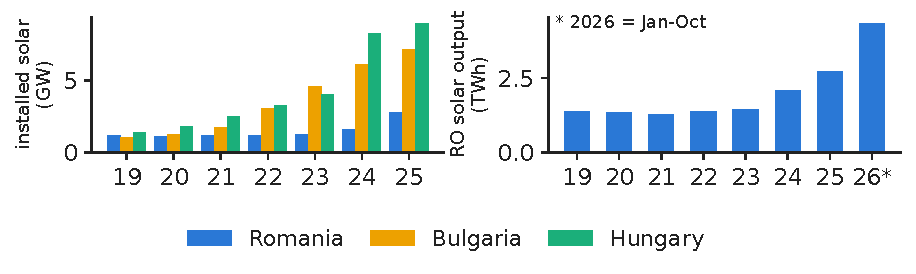
\includegraphics[width=\textwidth,height=0.526\textheight,keepaspectratio]{charts/en/solar_growth.pdf}\end{center}\vspace{-3mm}
\chartsource{Source: energy-charts.info (Fraunhofer ISE), installed capacity from ENTSO-E; ENTSO-E solar output (Transelectrica data). Data: installed capacity at year end 2019-2025; output 2019 to 2026-10-31.}
\vspace{0.5mm}
\begin{itemize}\setlength{\itemsep}{0pt}
  \item \textbf{Romanian solar output, Jan--Oct}: 2.53 TWh in 2025, 4.32 TWh in 2026
    \begin{itemize}\setlength{\itemsep}{0pt}
      \item 2.3\% of load in 2019, 10.2\% in 2026; neighbours: Bulgaria 7.2 GW, Hungary 9.0 GW
    \end{itemize}
\end{itemize}
\par\vfill\manager{a new solar park sells in the same sunny hours as every park already built, here and next door.}\par\vspace{0.5mm}
\par\vfill\noindent{\scriptsize\color{FooterGray}(ENTSO-E; metered output may omit rooftop panels)}\hfill\qlink{EMQA\_L6\_solar\_growth}{Quantlets/L6/EMQA_L6_solar_growth}\par\vspace{0.5mm}
\end{frame}

\subsection{The merit-order effect}

\begin{frame}{Zero-cost supply shifts the supply curve right and lowers the clearing price}
\footnotesize
\intuition{Solar and wind bid near zero, so dearer offers move right and the crossing with demand slides down.}
\begin{columns}[T,onlytextwidth]
\begin{column}{0.50\textwidth}
\[ S(p)+X\cdot\mathbf 1[p\ge 0]=D(p)\ \Rightarrow\ p^*(X) \]\vspace{-2mm}\[ \frac{\mathrm dp^*}{\mathrm dX}=-\frac{1}{S'(p^*)-D'(p^*)} \]{\footnotesize\begin{itemize}\setlength{\itemsep}{0pt}
  \item \textbf{\txtwhere}
    \begin{itemize}\setlength{\itemsep}{0pt}
      \item $S(p)$ = MW offered at prices $\le p$
      \item $D(p)$ = MW bid at prices $\ge p$
      \item $X$ = extra MW offered at 0 EUR/MWh
      \item $S'$, $D'$ = slopes of the curves (MW per EUR/MWh).
    \end{itemize}
\end{itemize}\par}
\end{column}
\begin{column}{0.47\textwidth}
\begin{itemize}\setlength{\itemsep}{2pt}
  \item \textbf{Reading the formula}
    \begin{itemize}\setlength{\itemsep}{0pt}
      \item Flat curves around the price: small effect
      \item Steep curves: large effect
    \end{itemize}
  \item \textbf{OPCOM, 21 Oct 2026, 12:00--12:15}
    \begin{itemize}\setlength{\itemsep}{0pt}
      \item Price 152.23 EUR/MWh
      \item Only 34 MW offered between 1 EUR/MWh and that price
    \end{itemize}
\end{itemize}
\end{column}
\end{columns}
\par\vfill\manager{the steeper the local curve, the more a new park moves its own price.}\par\vspace{0.5mm}
\par\vfill\noindent{\scriptsize\color{FooterGray}(Sensfuß, Ragwitz \& Genoese, 2008, ENPOL)}\hfill\tryit{notebook \S2}\par\vspace{0.5mm}
\end{frame}

\begin{frame}{On the Romanian order book alone, 40 MW more at zero price pushes midday below 50 EUR/MWh}
\footnotesize
\begin{center}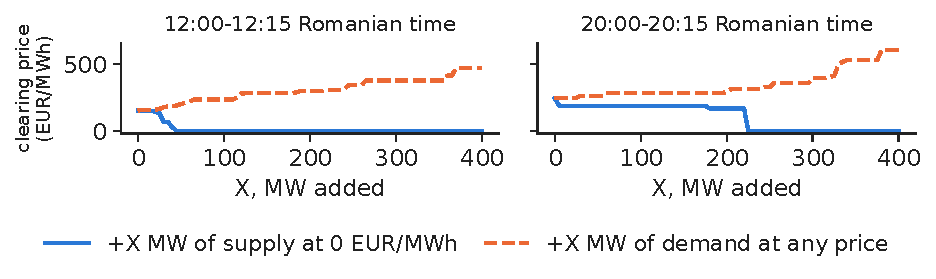
\includegraphics[width=\textwidth,height=0.406\textheight,keepaspectratio]{charts/en/merit_shift.pdf}\end{center}\vspace{-3mm}
\chartsource{Source: OPCOM, PZU aggregated curves (XML), own computation. Data: delivery day 2026-10-21; cross-border flows, blocks and hourly orders held at their accepted values.}
\vspace{0.5mm}
\begin{itemize}\setlength{\itemsep}{0pt}
  \item \textbf{Midday}: +25 MW at zero price, 152.23 $\to$ 131.40 EUR/MWh
    \begin{itemize}\setlength{\itemsep}{0pt}
      \item Evening: 1\,054 MW of net imports deepen the curve; 225 MW are needed for the same fall
      \item Flows held fixed, so this is an upper bound for the coupled market
    \end{itemize}
\end{itemize}
\par\vfill\manager{for Transelectrica: interconnectors, not local plants, give the midday price its depth.}\par\vspace{0.5mm}
\par\vfill\noindent{\scriptsize\color{FooterGray}(OPCOM aggregated curves; own computation)}\hfill\qlink{EMQA\_L6\_merit\_shift}{Quantlets/L6/EMQA_L6_merit_shift}\par\vspace{0.5mm}
\end{frame}

\begin{frame}{In the coupled market, 1 GW more solar lowers the Romanian price by about 27 EUR/MWh}
\footnotesize
\intuition{Within the same month and clock hour, sunnier and windier hours are cheaper; the regression measures by how much.}
\begin{columns}[T,onlytextwidth]
\begin{column}{0.49\textwidth}
\[ P_t=\underbrace{\alpha_{m(t)}+\gamma_{h(t)}+\delta_{w(t)}}_{\text{fixed effects}}+\beta_L L_t+\beta_W W_t+\beta_S S_t+\varepsilon_t \]{\footnotesize\begin{itemize}\setlength{\itemsep}{0pt}
  \item \textbf{\txtwhere}
    \begin{itemize}\setlength{\itemsep}{0pt}
      \item $P_t$ = hourly price (EUR/MWh), $L_t$, $W_t$, $S_t$ = load, wind, solar (GW)
      \item $\alpha$, $\gamma$, $\delta$ = constants per month (fuel, carbon), clock hour and weekday, estimated by ordinary least squares (OLS).
    \end{itemize}
\end{itemize}\par}
\end{column}
\begin{column}{0.48\textwidth}
\begin{itemize}\setlength{\itemsep}{2pt}
  \item \textbf{Estimates}, 33\,600 hours, 2023 -- Oct 2026, $R^2$ = 0.65
    \begin{itemize}\setlength{\itemsep}{0pt}
      \item EUR/MWh per GW: solar \ensuremath{-}26.7, wind \ensuremath{-}15.3, load \ensuremath{+}40.7
      \item Standard error (SE) of solar 2.2, heteroskedasticity- and autocorrelation-consistent (HAC)
    \end{itemize}
  \item \textbf{At midday in 2026}
    \begin{itemize}\setlength{\itemsep}{0pt}
      \item 1.62 GW of solar: \ensuremath{-}43.3 EUR/MWh, an association, not a causal effect
    \end{itemize}
\end{itemize}
\end{column}
\end{columns}
\par\vfill\manager{a supplier buying midday blocks should expect them cheaper on sunny days, by about this amount.}\par\vspace{0.5mm}
\par\vfill\noindent{\scriptsize\color{FooterGray}(Cludius et al., 2014, ENEECO; Würzburg et al., 2013, ENEECO)}\hfill\tryit{notebook \S3}\par\vspace{0.5mm}
\end{frame}

\begin{frame}{Price rises with residual load; hours below 2 GW of residual load reached 9.0\% in 2026}
\footnotesize
\begin{center}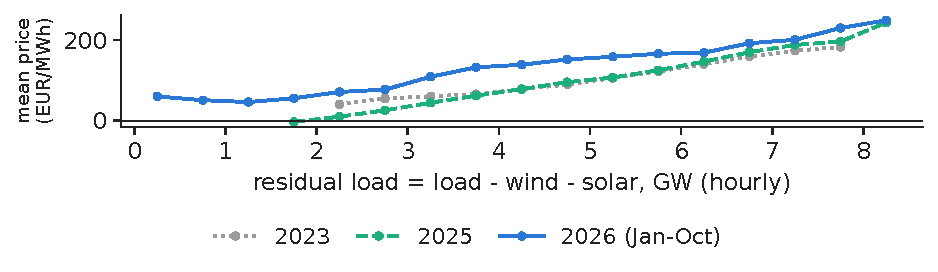
\includegraphics[width=\textwidth,height=0.423\textheight,keepaspectratio]{charts/en/resid_price.pdf}\end{center}\vspace{-3mm}
\chartsource{Source: energy-charts.info (Fraunhofer ISE); OPCOM prices; ENTSO-E solar, wind and load (Transelectrica data for Romania). Data: hourly, 2023-01-01 to 2026-10-31; bins of 0.5 GW with at least 20 hours.}
\vspace{0.5mm}
\begin{itemize}\setlength{\itemsep}{0pt}
  \item \textbf{Residual load} = load $-$ wind $-$ solar, the demand left for other plants and imports
    \begin{itemize}\setlength{\itemsep}{0pt}
      \item +1 GW raises the price by 28.3 EUR/MWh (SE 0.9), same fixed effects
      \item Hours below 2 GW: 0.1\% in 2023, 9.0\% in 2026
    \end{itemize}
\end{itemize}
\par\vfill\manager{a hydro producer saves water for high residual load, where each GW is worth most.}\par\vspace{0.5mm}
\par\vfill\noindent{\scriptsize\color{FooterGray}(own computation)}\hfill\qlink{EMQA\_L6\_resid\_price}{Quantlets/L6/EMQA_L6_resid_price}\par\vspace{0.5mm}
\end{frame}

\subsection{Renewables and the grid: redispatch}

\begin{frame}{Research from our group: machine learning forecasts German redispatch one day ahead}
\footnotesize
\begin{itemize}\setlength{\itemsep}{2pt}
  \item \textbf{Why redispatch}: wind in the north, demand in the industrial south of Germany
    \begin{itemize}\setlength{\itemsep}{0pt}
      \item After the day-ahead market, transmission system operators order plants up or down to keep lines within limits
    \end{itemize}
  \item \textbf{What the work did}: forecast the hourly redispatch volume (MW), up and down, of the four German operators
    \begin{itemize}\setlength{\itemsep}{0pt}
      \item 24 h ahead, with what is known on the afternoon of $d-1$: wind, solar, load, price spreads, scheduled exchanges
      \item Data Oct 2021 -- Feb 2026; 11 monthly test windows, Mar 2025 -- Feb 2026
    \end{itemize}
  \item \textbf{What it found}: deep neural networks are most often among the best models
    \begin{itemize}\setlength{\itemsep}{0pt}
      \item The best of them is in the model confidence set (mean absolute error) for 6 of the 8 series
      \item Covariates help only when aligned in time: significantly better forecasts in 40--60\% of the dense series
    \end{itemize}
\end{itemize}
\par\vfill\manager{for Transelectrica: forecast where wind and solar will meet the limits of the grid, a day ahead.}\par\vspace{0.5mm}
\par\vfill\noindent{\scriptsize\color{FooterGray}(Basangova, Bolovăneanu, Conda, Erlwein-Sayer, Melzer, Pele, Petukhina \& Phan, 2026, talk at AIDA 2026 (AI and Digital Assets in Energy and Finance), Bucharest, 3 June 2026: \href{https://github.com/danpele/EMQA/blob/main/resources/aida2026/bolovaneanu_redispatch_forecasting.pdf}{slides})}\par\vspace{0.5mm}
\end{frame}


\section{Capture prices and cannibalisation}

\subsection{Definitions}

\begin{frame}{The capture price is the average price weighted by the plant's own output}
\footnotesize
\intuition{A solar park is paid the price of the intervals in which it produces, not the average of all intervals.}
\begin{columns}[T,onlytextwidth]
\begin{column}{0.50\textwidth}
\[ \mathrm{CP}=\frac{\sum_t P_t G_t\Delta_t}{\sum_t G_t\Delta_t},\qquad B=\frac{\sum_t P_t\Delta_t}{\sum_t\Delta_t} \]\[ \mathrm{CR}=\frac{\mathrm{CP}}{B}=1+\frac{\mathrm{Cov}_\Delta(P,G)}{\bar P\,\bar G} \]{\footnotesize\begin{itemize}\setlength{\itemsep}{0pt}
  \item \textbf{\txtwhere}
    \begin{itemize}\setlength{\itemsep}{0pt}
      \item Capture price (CP), baseload price $B$, capture rate (CR)
      \item $P_t$ = price, $G_t$ = output (MW), $\Delta_t$ = 1 h or 0.25 h, $\mathrm{Cov}_\Delta$ = duration-weighted covariance (Appendix A).
    \end{itemize}
\end{itemize}\par}
\end{column}
\begin{column}{0.47\textwidth}
\begin{itemize}\setlength{\itemsep}{2pt}
  \item \textbf{Romanian solar, Jan--Oct 2026}
    \begin{itemize}\setlength{\itemsep}{0pt}
      \item CP 85.0, $B$ 137.5 EUR/MWh; CR 61.9\%
      \item Correlation of price and output \ensuremath{-}0.43: this pulls CR below 1
    \end{itemize}
  \item \textbf{Romanian wind, same period}
    \begin{itemize}\setlength{\itemsep}{0pt}
      \item CR 103.0\%: wind also blows at night and in winter
    \end{itemize}
\end{itemize}
\end{column}
\end{columns}
\par\vfill\manager{price a solar power purchase agreement (PPA) on the capture price, not on the baseload price.}\par\vspace{0.5mm}
\par\vfill\noindent{\scriptsize\color{FooterGray}(Hirth, 2013, ENEECO; Hirth, Ueckerdt \& Edenhofer, 2016, Energy J.)}\hfill\tryit{notebook \S4}\par\vspace{0.5mm}
\end{frame}

\subsection{Romania, year by year}

\begin{frame}{Solar's capture rate in Romania fell from 104\% in 2019 to 59\% in 2025}
\footnotesize
\begin{center}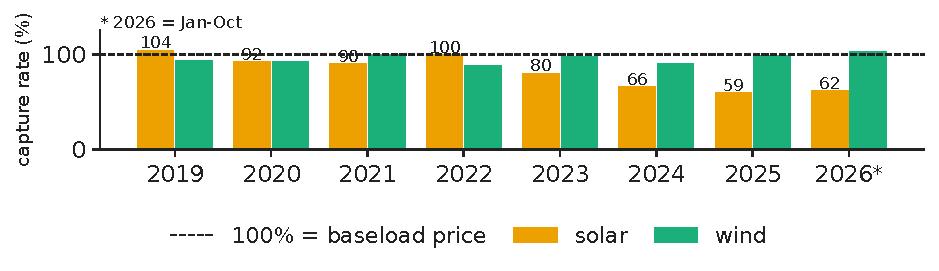
\includegraphics[width=\textwidth,height=0.477\textheight,keepaspectratio]{charts/en/capture_rates.pdf}\end{center}\vspace{-3mm}
\chartsource{Source: energy-charts.info (Fraunhofer ISE); OPCOM prices; ENTSO-E solar, wind and load (Transelectrica data for Romania). Data: 2019 to 2026-10-31; hourly to Sep 2025, 15-min from Oct 2025.}
\vspace{0.5mm}
\begin{itemize}\setlength{\itemsep}{0pt}
  \item \textbf{Solar}: the fall starts in 2023, with the growth of output
    \begin{itemize}\setlength{\itemsep}{0pt}
      \item 2026: 61.9\%, while output rose 71\% on the same months of 2025
      \item Wind: between 88\% and 103\%, no trend, because wind output did not grow
    \end{itemize}
\end{itemize}
\par\vfill\manager{a bank lending to a solar project should multiply the baseload price by the capture rate.}\par\vspace{0.5mm}
\par\vfill\noindent{\scriptsize\color{FooterGray}(own computation)}\hfill\qlink{EMQA\_L6\_capture\_rates}{Quantlets/L6/EMQA_L6_capture_rates}\par\vspace{0.5mm}
\end{frame}

\begin{frame}{In 2025 a Romanian solar MWh earned 43.9 EUR less than the baseload price}
\footnotesize
\begin{center}{\footnotesize\renewcommand{\arraystretch}{1.05}\setlength{\tabcolsep}{4pt}
\begin{tabular}{@{}lrrrrrrrr@{}}\toprule
Year & $B$ & Solar CP & Solar CR, \% & $B-\mathrm{CP}$ & Wind CP & Wind CR, \% & Solar TWh & Wind TWh \\ \midrule
2019 & 50.4 & 52.7 & \cellcolor{Forest!54}104.5 & \ensuremath{-}2.3 & 47.2 & \cellcolor{Forest!30}93.6 & 1.37 & 6.68 \\
2020 & 39.5 & 36.4 & \cellcolor{Forest!27}92.2 & \ensuremath{+}3.1 & 36.6 & \cellcolor{Forest!28}92.6 & 1.34 & 6.89 \\
2021 & 111.4 & 100.6 & \cellcolor{Forest!23}90.3 & \ensuremath{+}10.8 & 111.0 & \cellcolor{Forest!43}99.6 & 1.29 & 6.44 \\
2022 & 265.3 & 264.0 & \cellcolor{Forest!43}99.5 & \ensuremath{+}1.3 & 234.4 & \cellcolor{Forest!18}88.4 & 1.37 & 6.92 \\
2023 & 103.7 & 83.2 & 80.2 & \ensuremath{+}20.6 & 101.0 & \cellcolor{Forest!38}97.4 & 1.46 & 7.45 \\
2024 & 103.5 & 68.0 & \cellcolor{Crimson!31}65.7 & \ensuremath{+}35.5 & 93.4 & \cellcolor{Forest!22}90.2 & 2.09 & 6.34 \\
2025 & 108.2 & 64.2 & \cellcolor{Crimson!45}59.4 & \ensuremath{+}43.9 & 106.7 & \cellcolor{Forest!41}98.7 & 2.72 & 5.88 \\
2026* & 137.5 & 85.0 & \cellcolor{Crimson!40}61.9 & \ensuremath{+}52.4 & 141.6 & \cellcolor{Forest!51}103.0 & 4.32 & 5.27 \\
\bottomrule\end{tabular}}\end{center}\vspace{-2mm}\begin{itemize}\setlength{\itemsep}{1pt}
  \item \textbf{Reading the table}: $B$, CP in EUR/MWh; green = CR close to 100\%, red = far below
    \begin{itemize}\setlength{\itemsep}{0pt}
      \item * 2026 = Jan--Oct 2026; 2022 = energy crisis, all prices high
    \end{itemize}
\end{itemize}
\par\vfill\manager{the gap $B-\mathrm{CP}$ is a cost borne by the solar developer
    \begin{itemize}\setlength{\itemsep}{0pt}
      \item It grew every year since 2022.
    \end{itemize}}\par\vspace{0.5mm}
\par\vfill\noindent{\scriptsize\color{FooterGray}(own computation)}\hfill\tryit{notebook \S4}\par\vspace{0.5mm}
\end{frame}

\subsection{Cannibalisation}

\begin{frame}{When solar's share of monthly load rises by one point, the solar capture rate falls by about 4.2 points}
\footnotesize
\begin{center}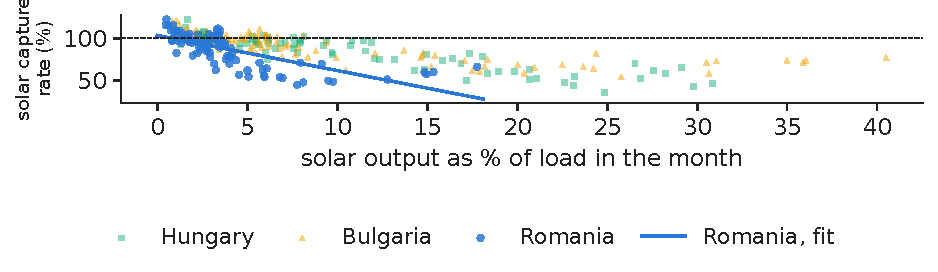
\includegraphics[width=\textwidth,height=0.423\textheight,keepaspectratio]{charts/en/cannibal.pdf}\end{center}\vspace{-3mm}
\chartsource{Source: energy-charts.info (Fraunhofer ISE); day-ahead prices (OPCOM, IBEX, HUPX); ENTSO-E solar output and load. Data: monthly, 2019-01 to 2026-10; Hungary from Oct 2019.}
\vspace{0.5mm}
\begin{itemize}\setlength{\itemsep}{0pt}
  \item \textbf{Regression} $\mathrm{CR}_m=a+b\,s_m+u_m$, $s_m$ = solar output as \% of load in month $m$
    \begin{itemize}\setlength{\itemsep}{0pt}
      \item Romania: $\hat b$ = \ensuremath{-}4.20 (SE 1.03), $R^2$ = 0.53, 94 months
      \item Hungary \ensuremath{-}2.14, Bulgaria \ensuremath{-}1.32: Romanian prices also fall with the neighbours' solar
    \end{itemize}
\end{itemize}
\par\vfill\manager{forecast regional solar, not only Romanian solar, to forecast a park's revenue.}\par\vspace{0.5mm}
\par\vfill\noindent{\scriptsize\color{FooterGray}(López Prol, Steininger \& Zilberman, 2020, ENEECO)}\hfill\qlink{EMQA\_L6\_cannibal}{Quantlets/L6/EMQA_L6_cannibal}\par\vspace{0.5mm}
\end{frame}

\begin{frame}{The region cannibalises together: Romanian, Bulgarian and Hungarian capture rates fell in step}
\footnotesize
\begin{center}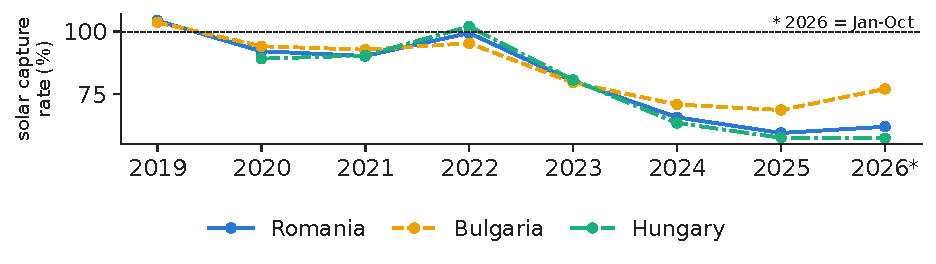
\includegraphics[width=\textwidth,height=0.462\textheight,keepaspectratio]{charts/en/capture_region.pdf}\end{center}\vspace{-3mm}
\chartsource{Source: energy-charts.info (Fraunhofer ISE); day-ahead prices (OPCOM, IBEX, HUPX); ENTSO-E solar output and load. Data: 2019 (Hungary 2020) to 2026-10-31; Bulgaria: hourly solar output.}
\vspace{0.5mm}
\begin{itemize}\setlength{\itemsep}{0pt}
  \item \textbf{2025}: Romania 59.4\%, Bulgaria 68.6\%, Hungary 57.5\%
    \begin{itemize}\setlength{\itemsep}{0pt}
      \item 2026: Bulgaria rises to 77.1\% as its battery fleet grows, an association, not a proof
    \end{itemize}
\end{itemize}
\par\vfill\manager{batteries charging at midday raise the price solar sells at: solar gains from other people's batteries.}\par\vspace{0.5mm}
\par\vfill\noindent{\scriptsize\color{FooterGray}(own computation; Bulgarian output is hourly)}\hfill\qlink{EMQA\_L6\_capture\_region}{Quantlets/L6/EMQA_L6_capture_region}\par\vspace{0.5mm}
\end{frame}

\begin{frame}{In 2025, 32.1\% of Romanian solar output was sold in the cheapest 10\% of hours}
\footnotesize
\begin{center}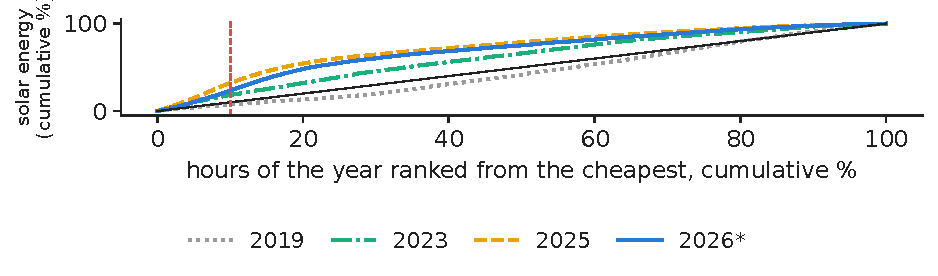
\includegraphics[width=\textwidth,height=0.406\textheight,keepaspectratio]{charts/en/cheap_hours.pdf}\end{center}\vspace{-3mm}
\chartsource{Source: energy-charts.info (Fraunhofer ISE); OPCOM prices; ENTSO-E solar, wind and load (Transelectrica data for Romania). Data: each calendar year; 2026 to 2026-10-31.}
\vspace{0.5mm}
\begin{itemize}\setlength{\itemsep}{0pt}
  \item \textbf{Reading}: hours ranked from the cheapest; the curve = share of the year's solar energy produced up to that rank
    \begin{itemize}\setlength{\itemsep}{0pt}
      \item 2019: 7.6\%; 2025: 32.1\%; 2026: 23.4\%; at zero or negative prices: 9.6\% of 2025 output
    \end{itemize}
\end{itemize}
\par\vfill\manager{as announced in Lecture 1: a solar park without storage sells much of its output in the cheapest hours of the year.}\par\vspace{0.5mm}
\par\vfill\noindent{\scriptsize\color{FooterGray}(own computation)}\hfill\qlink{EMQA\_L6\_cheap\_hours}{Quantlets/L6/EMQA_L6_cheap_hours}\par\vspace{0.5mm}
\end{frame}


\section{Negative prices}

\begin{frame}{A producer bids below zero when stopping costs more than paying to produce}
\footnotesize
\intuition{The bid is the cost of one more MWh minus what the plant earns or saves only by running.}
\begin{columns}[T,onlytextwidth]
\begin{column}{0.44\textwidth}
\[ b_i=c_i-s_i-k_i,\qquad h^{-}=\textstyle\sum_t \Delta_t\,\mathbf 1[P_t<0] \]{\footnotesize\begin{itemize}\setlength{\itemsep}{0pt}
  \item \textbf{\txtwhere}
    \begin{itemize}\setlength{\itemsep}{0pt}
      \item $b_i$ = offer of plant $i$ (EUR/MWh), $c_i$ = marginal cost
      \item $s_i$ = support paid per MWh produced, $k_i$ = restart cost per MWh of a stop
      \item $h^-$ = negative hours in hour-equivalents.
    \end{itemize}
\end{itemize}\par}
\end{column}
\begin{column}{0.53\textwidth}
\begin{itemize}\setlength{\itemsep}{2pt}
  \item \textbf{Who bids below zero}
    \begin{itemize}\setlength{\itemsep}{0pt}
      \item Output paid per MWh by a support scheme or contract
      \item Nuclear and run-of-river hydro, which cannot stop cheaply
    \end{itemize}
  \item \textbf{Romania, 2025}
    \begin{itemize}\setlength{\itemsep}{0pt}
      \item 196 negative hours; mean negative price \ensuremath{-}10.5 EUR/MWh
      \item Lowest 2026 price: \ensuremath{-}99.75 EUR/MWh
    \end{itemize}
\end{itemize}
\end{column}
\end{columns}
\par\vfill\manager{a merchant solar park has $b_i\approx 0$: it should stop as soon as the price turns negative.}\par\vspace{0.5mm}
\par\vfill\noindent{\scriptsize\color{FooterGray}(Fanone, Gamba \& Prokopczuk, 2013, ENEECO)}\hfill\tryit{notebook \S5}\par\vspace{0.5mm}
\end{frame}

\begin{frame}{Romania had 196 negative hours in 2025, Germany 575}
\footnotesize
\begin{center}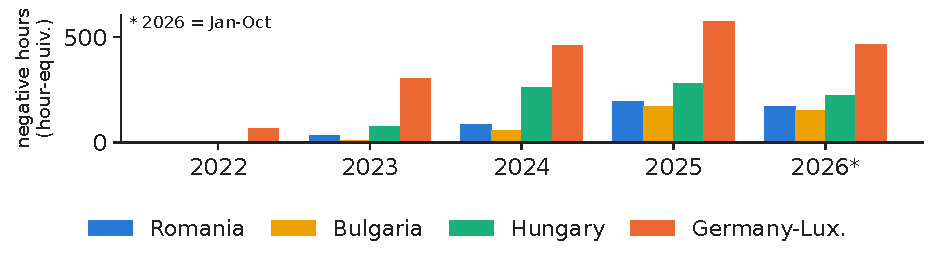
\includegraphics[width=\textwidth,height=0.525\textheight,keepaspectratio]{charts/en/neg_hours.pdf}\end{center}\vspace{-3mm}
\chartsource{Source: energy-charts.info (Fraunhofer ISE); day-ahead prices of OPCOM (RO), IBEX (BG), HUPX (HU), EPEX SPOT (DE-LU), via ENTSO-E. Data: 2022 to 2026-10-31; a 15-min interval counts 0.25 h.}
\vspace{0.5mm}
\begin{itemize}\setlength{\itemsep}{0pt}
  \item \textbf{Jan--Oct, 2025 vs 2026}: Romania 196 $\to$ 171.75 h, Hungary 281 $\to$ 223.5 h
    \begin{itemize}\setlength{\itemsep}{0pt}
      \item Fewer despite more solar; possible reasons: a higher price level, more batteries charging at midday
    \end{itemize}
\end{itemize}
\par\vfill\manager{a supplier with flexible industrial clients can be paid to consume in these hours.}\par\vspace{0.5mm}
\par\vfill\noindent{\scriptsize\color{FooterGray}(own computation; counting rule of Lecture 1)}\hfill\qlink{EMQA\_L6\_neg\_hours}{Quantlets/L6/EMQA_L6_neg_hours}\par\vspace{0.5mm}
\end{frame}

\begin{frame}{Switching off at negative prices saves little; the low positive midday price is the real loss}
\footnotesize
\intuition{A merchant park gains $|P_t|$ for each MWh it does not produce at a negative price; such MWh are few.}
\begin{columns}[T,onlytextwidth]
\begin{column}{0.50\textwidth}
\[ g=\frac{\sum_t \max(0,-P_t)\,G_t\Delta_t}{\sum_t G_t\Delta_t}\quad\text{vs}\quad B-\mathrm{CP} \]{\footnotesize\begin{itemize}\setlength{\itemsep}{0pt}
  \item \textbf{\txtwhere}
    \begin{itemize}\setlength{\itemsep}{0pt}
      \item $G_t$ = solar output (MW)
      \item $g$ = gain per MWh of yearly output if the park stops in every negative interval
      \item $B-\mathrm{CP}$ = profile discount.
    \end{itemize}
\end{itemize}\par}
\end{column}
\begin{column}{0.47\textwidth}
\begin{itemize}\setlength{\itemsep}{2pt}
  \item \textbf{Romanian solar, 2025}
    \begin{itemize}\setlength{\itemsep}{0pt}
      \item 6.2\% of output at negative prices, costing 1.71 million EUR
      \item $g$ = 0.63 against $B-\mathrm{CP}$ = 43.9 EUR/MWh
    \end{itemize}
  \item \textbf{2026}
    \begin{itemize}\setlength{\itemsep}{0pt}
      \item 4.0\% of output; $g$ = 0.35 EUR/MWh
    \end{itemize}
\end{itemize}
\end{column}
\end{columns}
\par\vfill\manager{install remote switch-off because it is cheap, but value a park on its capture price.}\par\vspace{0.5mm}
\par\vfill\noindent{\scriptsize\color{FooterGray}(own computation)}\hfill\tryit{notebook \S5}\par\vspace{0.5mm}
\end{frame}

\begin{frame}{Quarter-hours reveal 26 negative prices hidden inside hours with a non-negative average}
\footnotesize
\begin{itemize}\setlength{\itemsep}{4pt}
  \item \textbf{Since the 15-minute MTU of the Single Day-Ahead Coupling (SDAC)}, 1 Oct 2025
    \begin{itemize}\setlength{\itemsep}{0pt}
      \item 687 negative quarter-hours in Romania = 171.75 hour-equivalents
      \item 26 of them (3.8\%) fall in hours whose average is zero or positive
    \end{itemize}
  \item \textbf{Why it matters}
    \begin{itemize}\setlength{\itemsep}{0pt}
      \item Hourly averages show only 195 negative hours
      \item A battery or flexible load acting per quarter-hour can use them; a park metered per quarter-hour pays them
    \end{itemize}
  \item \textbf{Counting rule}
    \begin{itemize}\setlength{\itemsep}{0pt}
      \item $h^-=\sum_t\Delta_t\mathbf 1[P_t<0]$, $\Delta_t$ = 0.25 h: never count a quarter-hour as an hour
    \end{itemize}
\end{itemize}
\par\vfill\manager{set switch-off and battery logic on the 15-minute grid, as the market now is.}\par\vspace{0.5mm}
\par\vfill\noindent{\scriptsize\color{FooterGray}(NEMO Committee, 2025; own computation)}\hfill\tryit{notebook \S5}\par\vspace{0.5mm}
\end{frame}


\section{Intraday shape and price spreads}

\begin{frame}{Spring quarter-hours: 23.0 EUR/MWh at midday, 208.3 in the evening}
\footnotesize
\begin{center}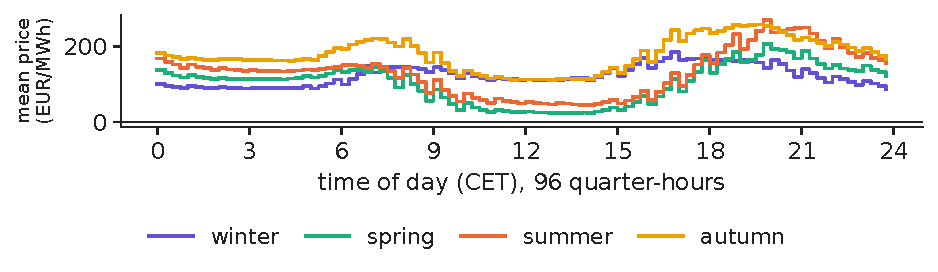
\includegraphics[width=\textwidth,height=0.533\textheight,keepaspectratio]{charts/en/shape15.pdf}\end{center}\vspace{-3mm}
\chartsource{Source: energy-charts.info (Fraunhofer ISE); OPCOM day-ahead prices for Romania, via ENTSO-E. Data: last 12 months 2025-11-01 to 2026-10-31, 15-min prices, CET; winter = Dec-Feb, spring = Mar-May, summer = Jun-Aug, autumn = Sep-Nov.}
\vspace{0.5mm}
\begin{itemize}\setlength{\itemsep}{0pt}
  \item \textbf{The solar valley}: spring minimum at 12:45, maximum at 19:45 CET
    \begin{itemize}\setlength{\itemsep}{0pt}
      \item Maximum minus minimum: spring 185, summer 226, winter only 98 EUR/MWh
    \end{itemize}
\end{itemize}
\par\vfill\manager{a battery charges in the valley and discharges on the evening ramp: the gap is its gross margin.}\par\vspace{0.5mm}
\par\vfill\noindent{\scriptsize\color{FooterGray}(own computation, last 12 months (Nov 2025 -- Oct 2026))}\hfill\qlink{EMQA\_L6\_shape15}{Quantlets/L6/EMQA_L6_shape15}\par\vspace{0.5mm}
\end{frame}

\begin{frame}{A battery earns the spread between dear and cheap hours, minus its losses}
\footnotesize
\intuition{Buy a MWh when it is cheap; sell what survives the round trip when it is dear.}
\begin{columns}[T,onlytextwidth]
\begin{column}{0.50\textwidth}
\[ S^{(k)}_d=\bar P^{\,\mathrm{top}\,k}_d-\bar P^{\,\mathrm{bot}\,k}_d \]\[ \pi_d\approx k\,\big(\eta\,\bar P^{\,\mathrm{top}\,k}_d-\bar P^{\,\mathrm{bot}\,k}_d\big) \]{\footnotesize\begin{itemize}\setlength{\itemsep}{0pt}
  \item \textbf{\txtwhere}
    \begin{itemize}\setlength{\itemsep}{0pt}
      \item $\bar P^{\,\mathrm{top}\,k}_d$, $\bar P^{\,\mathrm{bot}\,k}_d$ = mean price of the $k$ dearest and cheapest hours of day $d$, $k$ = hours of storage
      \item $\eta$ = round-trip efficiency (85\%), $\pi_d$ = gross margin of one cycle, 1 MW (EUR).
    \end{itemize}
\end{itemize}\par}
\end{column}
\begin{column}{0.47\textwidth}
\begin{itemize}\setlength{\itemsep}{2pt}
  \item \textbf{Romania, $k=2$, mean daily spread}
    \begin{itemize}\setlength{\itemsep}{0pt}
      \item 45 EUR/MWh in 2019, 151 in 2025, 174 in 2026
    \end{itemize}
  \item \textbf{Losses set a threshold}
    \begin{itemize}\setlength{\itemsep}{0pt}
      \item Buying at 50 EUR/MWh, it must sell above $50/0.85\approx59$ EUR/MWh
    \end{itemize}
\end{itemize}
\end{column}
\end{columns}
\par\vfill\manager{a battery developer reads the business case from the daily spread, before any model.}\par\vspace{0.5mm}
\par\vfill\noindent{\scriptsize\color{FooterGray}(Sioshansi et al., 2009, ENEECO)}\hfill\tryit{notebook \S6}\par\vspace{0.5mm}
\end{frame}

\begin{frame}{The daily spread is about four times its 2019 level and similar in Romania, Bulgaria and Hungary}
\footnotesize
\begin{center}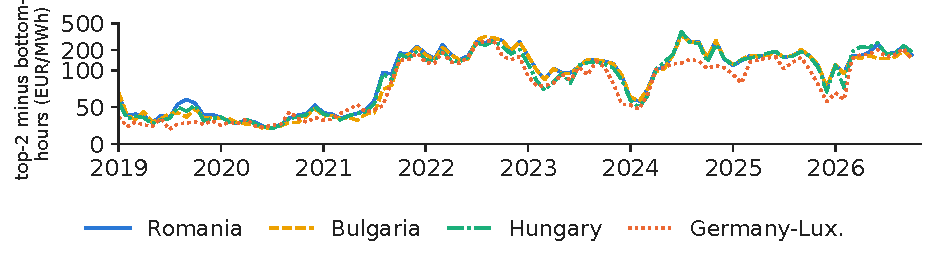
\includegraphics[width=\textwidth,height=0.459\textheight,keepaspectratio]{charts/en/spreads.pdf}\end{center}\vspace{-3mm}
\chartsource{Source: energy-charts.info (Fraunhofer ISE); day-ahead prices of OPCOM (RO), IBEX (BG), HUPX (HU), EPEX SPOT (DE-LU), via ENTSO-E. Data: daily, hourly prices (15-min averaged), monthly means, 2019 to 2026-10-31.}
\vspace{0.5mm}
\begin{itemize}\setlength{\itemsep}{0pt}
  \item \textbf{Dearest 2 minus cheapest 2 hours, 2026}: Romania 174, Bulgaria 150, Hungary 187, Germany 152 EUR/MWh
    \begin{itemize}\setlength{\itemsep}{0pt}
      \item Coupled markets: every battery in the region competes for the same spread
    \end{itemize}
\end{itemize}
\par\vfill\manager{treat the spread as a regional resource, shared with every new battery next door.}\par\vspace{0.5mm}
\par\vfill\noindent{\scriptsize\color{FooterGray}(own computation)}\hfill\qlink{EMQA\_L6\_spreads}{Quantlets/L6/EMQA_L6_spreads}\par\vspace{0.5mm}
\end{frame}


\section{The economics of a battery}

\subsection{The optimal schedule}

\begin{frame}{The best daily schedule of a battery solves a small linear programme}
\footnotesize
\intuition{Choose when to charge and discharge to maximise revenue, within the battery's physical limits.}
\begin{columns}[T,onlytextwidth]
\begin{column}{0.53\textwidth}
\[ \max_{c,\,x}\ \textstyle\sum_t P_t\,(x_t-c_t)\,\Delta_t \]\vspace{-3mm}\[ e_t=e_{t-1}+\big(\sqrt\eta\,c_t-x_t/\sqrt\eta\big)\Delta_t \]\vspace{-3mm}\[ 0\le e_t\le E,\ e_0=e_T=0,\ 0\le c_t,x_t\le 1,\ \textstyle\sum_t x_t\Delta_t\le\sqrt\eta E \]{\footnotesize\begin{itemize}\setlength{\itemsep}{0pt}
  \item \textbf{\txtwhere}
    \begin{itemize}\setlength{\itemsep}{0pt}
      \item $c_t$, $x_t$ = charging, discharging power (MW)
      \item $e_t$ = stored energy (MWh)
      \item $E$ = 1, 2 or 4 MWh
      \item $\eta$ = 0.85
      \item Last constraint: at most one cycle a day (Appendix B).
    \end{itemize}
\end{itemize}\par}
\end{column}
\begin{column}{0.44\textwidth}
\begin{itemize}\setlength{\itemsep}{2pt}
  \item \textbf{Assumptions}
    \begin{itemize}\setlength{\itemsep}{0pt}
      \item 85\% round trip, one cycle a day: National Renewable Energy Laboratory (NREL) reference
      \item No capacity fade, fees or balancing revenue
    \end{itemize}
  \item \textbf{Two information sets}
    \begin{itemize}\setlength{\itemsep}{0pt}
      \item Perfect foresight: prices known, an upper bound
      \item Forecast rule: optimise on a forecast, get paid real prices
    \end{itemize}
\end{itemize}
\end{column}
\end{columns}
\par\vfill\manager{this programme, with your own prices and limits, is the core of every battery dispatch tool.}\par\vspace{0.5mm}
\par\vfill\noindent{\scriptsize\color{FooterGray}(Cole \& Karmakar, 2023, NREL)}\hfill\tryit{notebook \S7}\par\vspace{0.5mm}
\end{frame}

\begin{frame}{With perfect foresight, a 2-hour battery earned 111.2 thousand EUR per MW in the last 12 months}
\footnotesize
\begin{center}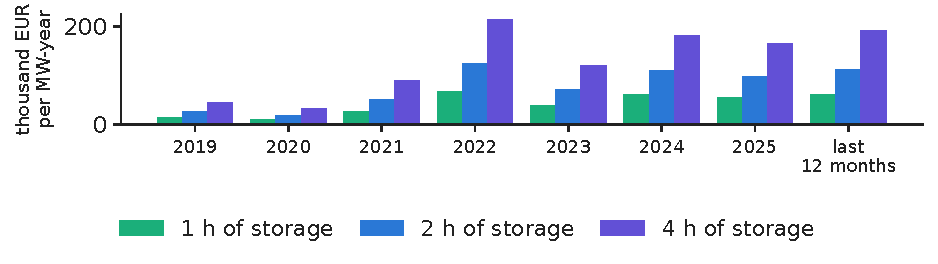
\includegraphics[width=\textwidth,height=0.459\textheight,keepaspectratio]{charts/en/bat_years.pdf}\end{center}\vspace{-3mm}
\chartsource{Source: energy-charts.info; day-ahead prices via ENTSO-E; ENTSO-E battery output (BG, RO); own optimisation. Data: 1 MW, round trip 85\%, max one cycle a day; 2019-2025 and last 12 months 2025-11-01 to 2026-10-31.}
\vspace{0.5mm}
\begin{itemize}\setlength{\itemsep}{0pt}
  \item \textbf{2 hours, thousand EUR per MW-year}: 26.3 (2019), 125.0 (2022), 98.7 (2025)
    \begin{itemize}\setlength{\itemsep}{0pt}
      \item 4 hours earn 1.72 times what 2 hours earn: the third and fourth hours trade a smaller spread
    \end{itemize}
\end{itemize}
\par\vfill\manager{size the battery on the revenue of each extra MWh of storage, not on total revenue.}\par\vspace{0.5mm}
\par\vfill\noindent{\scriptsize\color{FooterGray}(own computation; day-ahead prices only)}\hfill\qlink{EMQA\_L6\_bat\_years}{Quantlets/L6/EMQA_L6_bat_years}\par\vspace{0.5mm}
\end{frame}

\begin{frame}{A simple 7-day rule earns 85\% of the 2-hour perfect-foresight revenue}
\footnotesize
\begin{center}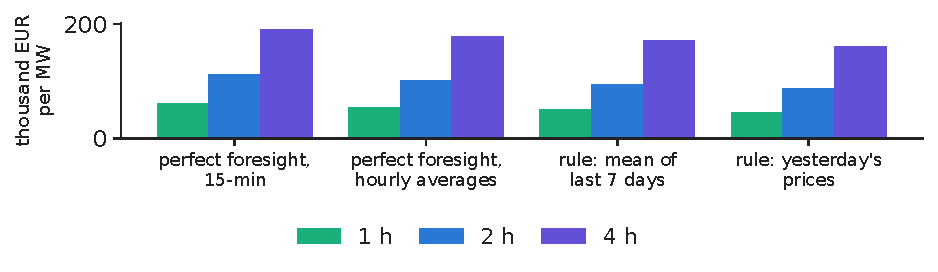
\includegraphics[width=\textwidth,height=0.531\textheight,keepaspectratio]{charts/en/bat_rules.pdf}\end{center}\vspace{-3mm}
\chartsource{Source: energy-charts.info; day-ahead prices via ENTSO-E; ENTSO-E battery output (BG, RO); own optimisation. Data: last 12 months 2025-11-01 to 2026-10-31; 1 MW, round trip 85\%; forecast rules on 361 common days, scaled to the full period.}
\vspace{0.5mm}
\begin{itemize}\setlength{\itemsep}{0pt}
  \item \textbf{Rules known at 12:00 CET on $d-1$}: mean profile of the last 7 days, 82\%, 85\%, 89\% (1, 2, 4 h)
    \begin{itemize}\setlength{\itemsep}{0pt}
      \item Yesterday's prices: 75\%, 79\%, 84\%; longer batteries forgive timing errors
    \end{itemize}
\end{itemize}
\par\vfill\manager{budget on a rule you can actually run: a better forecast (Lecture 2) closes part of the gap.}\par\vspace{0.5mm}
\par\vfill\noindent{\scriptsize\color{FooterGray}(own computation, last 12 months (Nov 2025 -- Oct 2026))}\hfill\qlink{EMQA\_L6\_bat\_rules}{Quantlets/L6/EMQA_L6_bat_rules}\par\vspace{0.5mm}
\end{frame}

\subsection{Probabilistic forecasts for trading}

\begin{frame}{Forecasting the whole price distribution helps a battery bid}
\footnotesize
\begin{itemize}\setlength{\itemsep}{2pt}
  \item \textbf{What the work did}: forecast the joint next-day distribution of 96 hourly prices (24 h $\times$ Romania, Bulgaria, Hungary, Czechia)
    \begin{itemize}\setlength{\itemsep}{0pt}
      \item Distributional random forest, 37 predictors, Jan 2018 -- Sep 2024; 70 rolling windows: 365 days to train, the next 30 to test
      \item The median picks the charge hour and the later discharge hour; quantiles set the buy and sell limit prices
    \end{itemize}
  \item \textbf{What it found}: forecast errors peak at 17:00--18:00, usually the discharge hours
    \begin{itemize}\setlength{\itemsep}{0pt}
      \item Romania, cumulative profit of a 1 MW / 1 MWh battery: 143.0 thousand EUR with the quantile rule, 133.2 with fixed hours, 188.2 with perfect foresight
      \item The quantile rule beats the fixed-hour rule in all four markets; trading across markets adds value (150.3 thousand EUR)
    \end{itemize}
  \item \textbf{Investment}: with 500\,000 EUR upfront, 90\% efficiency, 15 years and 7\%, day-ahead arbitrage alone does not cover it
\end{itemize}
\par\vfill\manager{bid from forecast quantiles, not from a single price forecast: the hours that pay are in the tails.}\par\vspace{0.5mm}
\par\vfill\noindent{\scriptsize\color{FooterGray}(Andrei, Cepoi, Dumitrescu, Lessmann, Luchian, Pele \& Petukhina, 2026, \href{https://doi.org/10.2139/ssrn.6872381}{doi:10.2139/ssrn.6872381}; talk by C.\,O.\ Cepoi at AIDA 2026, Bucharest, 3 June 2026: \href{https://github.com/danpele/EMQA/blob/main/resources/aida2026/cepoi_battery_arbitrage.pdf}{slides})}\par\vspace{0.5mm}
\end{frame}

\subsection{15 minutes, self-cannibalisation, the region}

\begin{frame}{15-minute prices raised a 1-hour battery's revenue by 14.5\% on the same days}
\footnotesize
\intuition{Any hourly schedule can be run on quarter-hours, so finer prices can only add revenue.}
\begin{columns}[T,onlytextwidth]
\begin{column}{0.50\textwidth}
\[ R^{15}=\max_{c,x}\textstyle\sum_t P^{15}_t(x_t-c_t)\tfrac14\ \ge\ R^{60} \]{\footnotesize\begin{itemize}\setlength{\itemsep}{0pt}
  \item \textbf{\txtwhere}
    \begin{itemize}\setlength{\itemsep}{0pt}
      \item $R^{15}$ = optimal revenue on the 96 quarter-hour prices $P^{15}_t$
      \item $R^{60}$ = optimal revenue when each hour is paid the mean of its quarters
      \item Same days, so the difference is the value of granularity alone.
    \end{itemize}
\end{itemize}\par}
\end{column}
\begin{column}{0.47\textwidth}
\begin{itemize}\setlength{\itemsep}{2pt}
  \item \textbf{Last 12 months, thousand EUR per MW}
    \begin{itemize}\setlength{\itemsep}{0pt}
      \item 1 h: 53.2 $\to$ 61.0 (\ensuremath{+}14.5\%)
      \item 2 h: 100.8 $\to$ 111.2 (\ensuremath{+}10.3\%)
      \item 4 h: 178.4 $\to$ 190.9 (\ensuremath{+}7.0\%)
    \end{itemize}
  \item A comparison with the hourly year before would mix in price-level changes.
\end{itemize}
\end{column}
\end{columns}
\par\vfill\manager{short batteries gain most from 15-minute prices.}\par\vspace{0.5mm}
\par\vfill\noindent{\scriptsize\color{FooterGray}(NEMO Committee, 2025; own computation)}\hfill\tryit{notebook \S8}\par\vspace{0.5mm}
\end{frame}

\begin{frame}{Batteries cannibalise their own spread: on the local order book, 50 MW would have closed it on 21 Oct 2026}
\footnotesize
\intuition{Charging adds demand at midday and discharging adds supply in the evening: both pull the two prices together.}
\begin{columns}[T,onlytextwidth]
\begin{column}{0.50\textwidth}
\[ \Delta P(X)=p^{*}_{\text{eve}}(+X\text{ supply})-p^{*}_{\text{mid}}(+X\text{ demand}) \]{\footnotesize\begin{itemize}\setlength{\itemsep}{0pt}
  \item \textbf{\txtwhere}
    \begin{itemize}\setlength{\itemsep}{0pt}
      \item $X$ = MW of batteries
      \item $p^*$ = clearing price recomputed on the OPCOM curves of 12:00--12:15 and 20:00--20:15 (Romanian time)
      \item Flows fixed (Appendix C).
    \end{itemize}
\end{itemize}\par}
\end{column}
\begin{column}{0.47\textwidth}
\begin{itemize}\setlength{\itemsep}{2pt}
  \item \textbf{Evening minus midday price}
    \begin{itemize}\setlength{\itemsep}{0pt}
      \item Actual 91.77 EUR/MWh
      \item 50 MW: \ensuremath{-}13.15; 100 MW: \ensuremath{-}47.12
    \end{itemize}
  \item \textbf{Fleets already running}
    \begin{itemize}\setlength{\itemsep}{0pt}
      \item Romania: battery output up to 766 MW in 2026
      \item Bulgaria, reported since 9 Sep 2026: up to 2\,795 MW
    \end{itemize}
\end{itemize}
\end{column}
\end{columns}
\par\vfill\manager{model the spread after the fleet is built, not the spread seen before it.}\par\vspace{0.5mm}
\par\vfill\noindent{\scriptsize\color{FooterGray}(OPCOM aggregated curves; own computation)}\hfill\tryit{notebook \S2}\par\vspace{0.5mm}
\end{frame}

\begin{frame}{A Romanian battery competes for the same regional spread as the Bulgarian and Hungarian ones}
\footnotesize
\begin{center}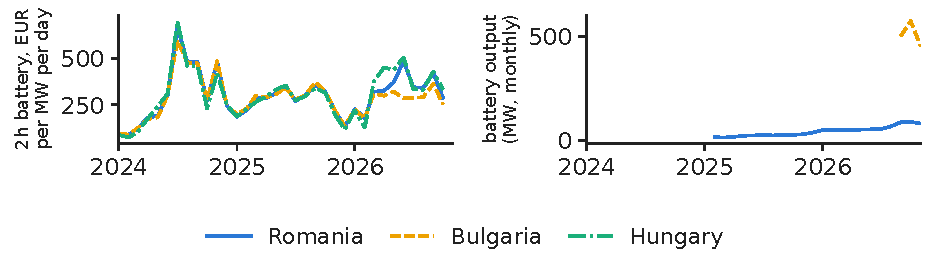
\includegraphics[width=\textwidth,height=0.412\textheight,keepaspectratio]{charts/en/bat_region.pdf}\end{center}\vspace{-3mm}
\chartsource{Source: energy-charts.info; day-ahead prices via ENTSO-E; ENTSO-E battery output (BG, RO); own optimisation. Data: 2h battery, perfect foresight, 2024-01 to 2026-10; battery output as reported to ENTSO-E.}
\vspace{0.5mm}
\begin{itemize}\setlength{\itemsep}{0pt}
  \item \textbf{2 hours, last 12 months, thousand EUR per MW}: Hungary 117.6, Romania 111.2, Bulgaria 96.4, Germany 90.6
    \begin{itemize}\setlength{\itemsep}{0pt}
      \item Daily revenue correlation with Romania: Bulgaria 0.80, Hungary 0.87
    \end{itemize}
\end{itemize}
\par\vfill\manager{as announced in Lecture 1: a Romanian battery developer competes for the same regional evening spread.}\par\vspace{0.5mm}
\par\vfill\noindent{\scriptsize\color{FooterGray}(own computation; battery output as reported to ENTSO-E)}\hfill\qlink{EMQA\_L6\_bat\_region}{Quantlets/L6/EMQA_L6_bat_region}\par\vspace{0.5mm}
\end{frame}

\begin{frame}{At 8\% over 15 years, the 2-hour revenue supports at most 808 EUR per kW}
\footnotesize
\intuition{The largest investment a yearly revenue can repay is that revenue times the annuity factor.}
\begin{columns}[T,onlytextwidth]
\begin{column}{0.47\textwidth}
\[ I^{\max}=R\cdot a(r,n) \]\[ a(r,n)=\sum_{j=1}^{n}(1+r)^{-j}=\frac{1-(1+r)^{-n}}{r} \]{\footnotesize\begin{itemize}\setlength{\itemsep}{0pt}
  \item \textbf{\txtwhere}
    \begin{itemize}\setlength{\itemsep}{0pt}
      \item $R$ = yearly revenue per MW (EUR), $r$ = 8\% (assumption), $n$ = 15 years (NREL), so $a$ = 8.56
      \item $I^{\max}/1\,000$ = EUR per kilowatt (kW), Appendix D.
    \end{itemize}
\end{itemize}\par}
\end{column}
\begin{column}{0.50\textwidth}
\begin{itemize}\setlength{\itemsep}{2pt}
  \item \textbf{2 hours, last 12 months}
    \begin{itemize}\setlength{\itemsep}{0pt}
      \item Perfect foresight: 952 EUR/kW
      \item 7-day rule: 808 EUR/kW = 404 EUR per kilowatt-hour (kWh)
    \end{itemize}
  \item \textbf{Not included}
    \begin{itemize}\setlength{\itemsep}{0pt}
      \item Operating costs, grid tariffs, fade: lower $I^{\max}$
      \item Balancing revenue raises it; new fleets shrink the spread
    \end{itemize}
\end{itemize}
\end{column}
\end{columns}
\par\vfill\manager{compare 404 EUR/kWh with the turnkey quote before anything else.}\par\vspace{0.5mm}
\par\vfill\noindent{\scriptsize\color{FooterGray}(Cole \& Karmakar, 2023, NREL; Schmidt et al., 2019, Joule)}\hfill\tryit{notebook \S8}\par\vspace{0.5mm}
\end{frame}


\section{Case studies: Apr 2026; summer 2026}

\subsection{Apr 2026: the most negative hours}

\begin{frame}{Case study: in the week of 20 Apr 2026, Romania had 24 negative hours and solar captured 42\%}
\footnotesize
\begin{center}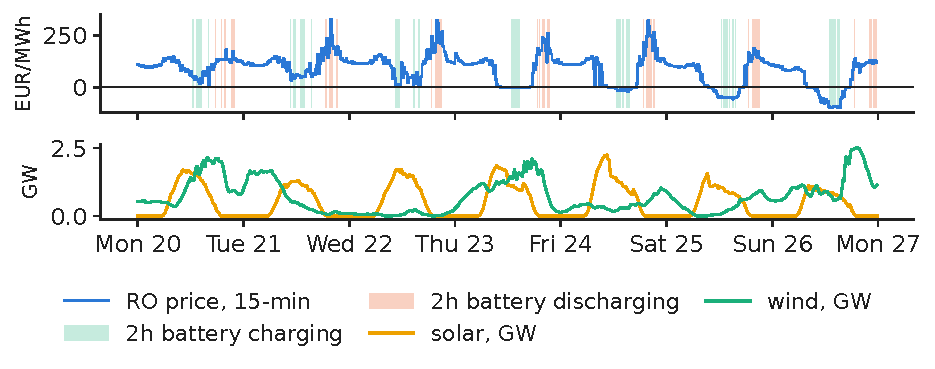
\includegraphics[width=\textwidth,height=0.469\textheight,keepaspectratio]{charts/en/case_week.pdf}\end{center}\vspace{-3mm}
\chartsource{Source: energy-charts.info (Fraunhofer ISE); OPCOM prices; ENTSO-E solar, wind and load (Transelectrica data for Romania). Data: week 2026-04-20 to 2026-04-26, 15-min, CET.}
\vspace{0.5mm}
\begin{itemize}\setlength{\itemsep}{0pt}
  \item \textbf{Prices from \ensuremath{-}99.75 to 328.00 EUR/MWh}; solar CP 37.0 vs $B$ 87.0
    \begin{itemize}\setlength{\itemsep}{0pt}
      \item 2-hour battery: 391 EUR per MW a day, against 305 on an average day of the last 12 months
    \end{itemize}
\end{itemize}
\par\vfill\manager{the same sunny week is the worst for a solar park and among the best for a battery.}\par\vspace{0.5mm}
\par\vfill\noindent{\scriptsize\color{FooterGray}(own computation; schedule with perfect foresight)}\hfill\qlink{EMQA\_L6\_case\_week}{Quantlets/L6/EMQA_L6_case_week}\par\vspace{0.5mm}
\end{frame}

\begin{frame}{Case study: what Apr 2026 meant for each player in the Romanian market}
\footnotesize
\begin{itemize}\setlength{\itemsep}{3pt}
  \item \textbf{Solar developer}: capture rate 49.4\% (47.2 vs 95.6 EUR/MWh)
    \begin{itemize}\setlength{\itemsep}{0pt}
      \item 17.9\% of output at negative prices; decision: storage on site, or a PPA that prices the solar profile
    \end{itemize}
  \item \textbf{Wind developer}: capture rate 97.8\%
    \begin{itemize}\setlength{\itemsep}{0pt}
      \item In Romania, wind is not the cannibalised technology
    \end{itemize}
  \item \textbf{Battery developer}: 2 hours, 325 EUR per MW a day
    \begin{itemize}\setlength{\itemsep}{0pt}
      \item Against 305 on average over the last 12 months
    \end{itemize}
  \item \textbf{Supplier and industrial consumer}: 67 negative hours
    \begin{itemize}\setlength{\itemsep}{0pt}
      \item Moving consumption to spring middays is paid
    \end{itemize}
  \item \textbf{Transelectrica}
    \begin{itemize}\setlength{\itemsep}{0pt}
      \item After sunset the evening ramp and the interconnectors set the price
    \end{itemize}
\end{itemize}
\par\vfill\noindent{\scriptsize\color{FooterGray}(own computation)}\hfill\tryit{notebook \S9}\par\vspace{0.5mm}
\end{frame}

\subsection{Summer 2026: Romania and Bulgaria}

\begin{frame}{Summer 2026: midday exports, evening imports from Bulgaria}
\footnotesize
\begin{center}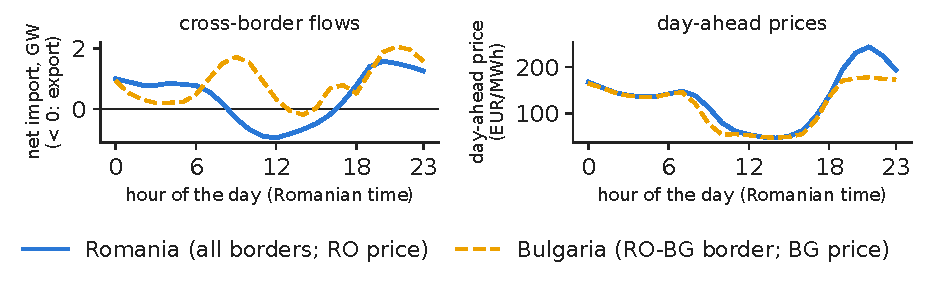
\includegraphics[width=\textwidth,height=0.430\textheight,keepaspectratio]{charts/en/rogb_summer.pdf}\end{center}\vspace{-3mm}
\chartsource{Source: energy-charts.info (Fraunhofer ISE): cross-border physical flows of Romania (ENTSO-E); day-ahead prices of OPCOM (RO) and IBEX (BG). Data: hourly means, 2026-06-01 to 2026-08-31; Moldova and Ukraine borders only partly reported.}
\vspace{0.5mm}
\begin{itemize}\setlength{\itemsep}{0pt}
  \item \textbf{Midday: Romania exports}, 960 MW net at 12:00 on all borders
    \begin{itemize}\setlength{\itemsep}{0pt}
      \item Mostly to Hungary (857 MW) and Serbia (367 MW); to Bulgaria on only 43 of 92 days (12:00--15:00)
    \end{itemize}
  \item \textbf{Evening: Romania imports from Bulgaria}, 2\,064 MW at 21:00, on all 92 days
    \begin{itemize}\setlength{\itemsep}{0pt}
      \item Price at 21:00: Romania 243.9, Bulgaria 178.3 EUR/MWh; the full border separates the two prices
    \end{itemize}
\end{itemize}
\par\vfill\manager{the evening gap of 65.6 EUR/MWh is the value of evening storage and interconnection.}\par\vspace{0.5mm}
\par\vfill\noindent{\scriptsize\color{FooterGray}(own computation; + = import into Romania)}\hfill\qlink{EMQA\_L6\_rogb\_summer}{Quantlets/L6/EMQA_L6_rogb_summer}\par\vspace{0.5mm}
\end{frame}

\section*{Wrap-up}

\begin{frame}{Quiz 1: capture rate}
\small
\begin{itemize}
  \item A solar PPA is offered at the 2025 baseload forward of 108 EUR/MWh
    \begin{itemize}\setlength{\itemsep}{0pt}
      \item What does the solar profile really earn?
    \end{itemize}
\end{itemize}
\vspace{2mm}
\begin{exampleblock}{Answer}
\begin{itemize}
  \item About 64 EUR/MWh in 2025 (capture rate 59\%)
    \begin{itemize}\setlength{\itemsep}{0pt}
      \item The buyer at the baseload price pays a large premium for the profile.
    \end{itemize}
\end{itemize}
\end{exampleblock}
\end{frame}

\begin{frame}{Quiz 2: counting negative prices}
\small
\begin{itemize}
  \item Since 1 October 2025, Romania has had 687 negative quarter-hours
    \begin{itemize}\setlength{\itemsep}{0pt}
      \item How many negative hours do you report?
    \end{itemize}
\end{itemize}
\vspace{2mm}
\begin{exampleblock}{Answer}
\begin{itemize}
  \item 171.75 hour-equivalents ($\times$0.25 h), not 687 hours.
\end{itemize}
\end{exampleblock}
\end{frame}

\begin{frame}{Quiz 3: battery duration}
\small
\begin{itemize}
  \item Doubling storage from 2 h to 4 h doubles the cost of the cells
    \begin{itemize}\setlength{\itemsep}{0pt}
      \item Does it double revenue?
    \end{itemize}
\end{itemize}
\vspace{2mm}
\begin{exampleblock}{Answer}
\begin{itemize}
  \item No: in the last 12 months a 4-hour battery earned 1.72 times what a 2-hour one earned, because the extra hours trade a smaller spread.
\end{itemize}
\end{exampleblock}
\end{frame}

\begin{frame}{Quiz 4: the merit-order effect}
\small
\begin{itemize}
  \item On the OPCOM curves of 21 Oct 2026, 25 MW more at zero price lowers the midday price to 131.4 EUR/MWh
    \begin{itemize}\setlength{\itemsep}{0pt}
      \item Is this what a new 25 MW park does?
    \end{itemize}
\end{itemize}
\vspace{2mm}
\begin{exampleblock}{Answer}
\begin{itemize}
  \item No: the curves hold cross-border flows fixed
    \begin{itemize}\setlength{\itemsep}{0pt}
      \item In the coupled market part of the extra output is exported, so the true effect is smaller (the regression gives a fall of about 27 EUR/MWh per GW).
    \end{itemize}
\end{itemize}
\end{exampleblock}
\end{frame}

\begin{frame}{Wrap-up}
\small
\vspace{-2mm}\begin{multicols}{2}\scriptsize\tableofcontents\end{multicols}
\begin{itemize}\setlength{\itemsep}{1pt}
  \item Solar lowers the price it is paid: Romanian capture rate 104\% (2019) $\to$ 59\% (2025)
    \begin{itemize}\setlength{\itemsep}{0pt}
      \item Wind near 100\%.
    \end{itemize}
  \item Batteries live on the same regional spread: 111 thousand EUR per MW for 2 h with perfect foresight, about 85\% of it with a simple rule
    \begin{itemize}\setlength{\itemsep}{0pt}
      \item Next: Lecture 7.
    \end{itemize}
\end{itemize}
\end{frame}

\begin{frame}{Research from our group on renewables and Romanian prices}
\footnotesize
\begin{itemize}\setlength{\itemsep}{2pt}
  \item \textbf{Explaining price drops and spikes} (Andrei \& Pele, 2025, Preprints)
    \begin{itemize}\setlength{\itemsep}{0pt}
      \item What the paper did: detected unusual hourly Romanian prices with an isolation forest and explained them with Shapley values
      \item Result: wind and solar output drive the price drops; load forecast errors and conventional generation drive the spikes
    \end{itemize}
  \item \textbf{Price drivers by horizon and regime} (Andrei, Pele \& Cramer, 2026, PICBE)
    \begin{itemize}\setlength{\itemsep}{0pt}
      \item What the paper did: forecast Romanian hourly prices 2018--2024 with tree ensembles and measured which drivers matter at each horizon and in low-, normal- and high-price regimes
      \item Use here: the renewable drivers behind the low-price regime of this lecture
    \end{itemize}
  \item \textbf{Early warning of spikes} (Andrei, Pele, Cramer, Amza \& Diaconu, 2026, PICBE)
    \begin{itemize}\setlength{\itemsep}{0pt}
      \item What the paper did: built an explainable artificial intelligence (AI) early-warning system for Romanian price spikes
      \item Result: the residual-load forecast is the main driver, the variable of our regression
    \end{itemize}
  \item \textbf{Price elasticity of demand} (Proșcanu, Proșcanu \& Pele, 2025, JSES)
    \begin{itemize}\setlength{\itemsep}{0pt}
      \item What the paper did: tested Granger causality between Romanian consumption and price
      \item Result: consumption does not react to price, hence the almost vertical demand curve of the merit order
    \end{itemize}
\end{itemize}
\par\vspace{0.5mm}{\scriptsize \begin{itemize}\setlength{\itemsep}{0pt}
  \item Findings as stated in the papers; numbers on the other slides come from our own data.
\end{itemize}}
\par\vfill\noindent{\scriptsize\color{FooterGray}(Bucharest University of Economic Studies; Romanian Academy, Institute for Economic Forecasting)}\par\vspace{0.5mm}
\end{frame}

\begin{frame}{Want to learn more?}
\small
\begin{columns}[T,onlytextwidth]
\begin{column}{0.52\textwidth}
\begin{itemize}\setlength{\itemsep}{4pt}
  \item \textbf{Hirth (2013)}: the reference paper on the value factor of wind and solar: \href{https://doi.org/10.1016/j.eneco.2013.02.004}{doi:10.1016/j.eneco.2013.02.004}.
  \item \textbf{Cole \& Karmakar (2023)}: battery costs, efficiency and lifetime used in this lecture: \href{https://doi.org/10.2172/1984976}{doi:10.2172/1984976}.
  \item \textbf{energy-charts.info}: live prices, generation and installed capacity for Romania and its neighbours: \href{https://energy-charts.info}{energy-charts.info}.
\end{itemize}
\end{column}
\begin{column}{0.45\textwidth}
\begin{itemize}\setlength{\itemsep}{4pt}
  \item \textbf{This course}: code, data, notebooks --- \href{https://github.com/danpele/EMQA}{github.com/danpele/EMQA}.
  \item \textbf{OPCOM aggregated curves}: download another day and repeat the merit-order computation: \href{https://www.opcom.ro/rapoarte-pzu-curbe-agregate/ro}{opcom.ro}.
  \item \textbf{Experiment yourself}: the notebook reproduces every chart and number of this lecture.
\end{itemize}
\end{column}
\end{columns}
\end{frame}

\begin{frame}{References (1/3)}
\scriptsize
\begin{itemize}\setlength{\itemsep}{1pt}\scriptsize
\item Andrei, A.-V.\ \& Pele, D.\,T.\ (2025). Explainable AI for electricity price anomaly detection: A SHAP-driven approach in Romania's energy market. \textit{Preprints}. \href{https://doi.org/10.20944/preprints202508.0410.v1}{doi:10.20944/preprints202508.0410.v1}
\item Andrei, A.-V., Cepoi, C., Dumitrescu, B.-A., Lessmann, S., Luchian, A., Pele, D.-T.\ \& Petukhina, A.\ (2026). Joint probabilistic forecasting for battery arbitrage in day-ahead power markets. SSRN Working Paper 6872381. \href{https://doi.org/10.2139/ssrn.6872381}{doi:10.2139/ssrn.6872381}
\item Andrei, A.-V., Pele, D.-T.\ \& Cramer, A.-A.\ (2026). Multi-horizon explainability in energy price forecasting: Disentangling market dynamics and renewable intermittency in Romania's liberalized electricity market. \textit{Proceedings of the International Conference on Business Excellence}, 20(1), 104--117. \href{https://doi.org/10.2478/picbe-2026-0014}{doi:10.2478/picbe-2026-0014}
\item Andrei, A.-V., Pele, D.-T., Cramer, A.-A., Amza, A.\ \& Diaconu, D.\ (2026). Explainable AI-based early warning system for electricity price spikes: Evidence from the Romanian market. \textit{Proceedings of the International Conference on Business Excellence}, 20(1), 4820--4836. \href{https://doi.org/10.2478/picbe-2026-0352}{doi:10.2478/picbe-2026-0352}
\item Basangova, M., Bolovăneanu, V., Conda, A., Erlwein-Sayer, C., Melzer, A., Pele, D.\,T., Petukhina, A.\ \& Phan, M.\ (2026). Day-ahead forecasting for redispatch measures using machine learning models. Talk at the AIDA Conference, Bucharest University of Economic Studies, 3 June 2026. \href{https://github.com/danpele/EMQA/blob/main/resources/aida2026/bolovaneanu_redispatch_forecasting.pdf}{github.com/danpele/EMQA}
\item Bradbury, K., Pratson, L.\ \& Patiño-Echeverri, D.\ (2014). Economic viability of energy storage systems based on price arbitrage potential in real-time U.S.\ electricity markets. \textit{Applied Energy}, 114, 512--519. \href{https://doi.org/10.1016/j.apenergy.2013.10.010}{doi:10.1016/j.apenergy.2013.10.010}
\item Cludius, J., Hermann, H., Matthes, F.\,C.\ \& Graichen, V.\ (2014). The merit order effect of wind and photovoltaic electricity generation in Germany 2008--2016: Estimation and distributional implications. \textit{Energy Economics}, 44, 302--313. \href{https://doi.org/10.1016/j.eneco.2014.04.020}{doi:10.1016/j.eneco.2014.04.020}
\end{itemize}
\end{frame}

\begin{frame}{References (2/3)}
\scriptsize
\begin{itemize}\setlength{\itemsep}{1pt}\scriptsize
\item Cepoi, C.\,O.\ (2026). Uncertainty meets opportunity: Joint probabilistic forecasting for battery arbitrage in CEE day-ahead power markets. Talk at the AIDA Conference, Bucharest University of Economic Studies, 3 June 2026. \href{https://github.com/danpele/EMQA/blob/main/resources/aida2026/cepoi_battery_arbitrage.pdf}{github.com/danpele/EMQA}
\item Cole, W.\ \& Karmakar, A.\ (2023). Cost projections for utility-scale battery storage: 2023 update. NREL/TP-6A40-85332, National Renewable Energy Laboratory. \href{https://doi.org/10.2172/1984976}{doi:10.2172/1984976}
\item Fanone, E., Gamba, A.\ \& Prokopczuk, M.\ (2013). The case of negative day-ahead electricity prices. \textit{Energy Economics}, 35, 22--34. \href{https://doi.org/10.1016/j.eneco.2011.12.006}{doi:10.1016/j.eneco.2011.12.006}
\item Hirth, L.\ (2013). The market value of variable renewables: The effect of solar wind power variability on their relative price. \textit{Energy Economics}, 38, 218--236. \href{https://doi.org/10.1016/j.eneco.2013.02.004}{doi:10.1016/j.eneco.2013.02.004}
\item Hirth, L., Ueckerdt, F.\ \& Edenhofer, O.\ (2016). Why wind is not coal: On the economics of electricity generation. \textit{The Energy Journal}, 37(3), 1--28. \href{https://doi.org/10.5547/01956574.37.3.lhir}{doi:10.5547/01956574.37.3.lhir}
\item López Prol, J., Steininger, K.\,W.\ \& Zilberman, D.\ (2020). The cannibalization effect of wind and solar in the California wholesale electricity market. \textit{Energy Economics}, 85, 104552. \href{https://doi.org/10.1016/j.eneco.2019.104552}{doi:10.1016/j.eneco.2019.104552}
\item NEMO Committee (2025). 15-Minute MTU in SDAC was implemented. Single Day-Ahead Coupling (SDAC) press release, 1 October 2025. \href{https://nemo-committee.eu/assets/files/15-minute-mtu-in-sdac-was-implemented.pdf}{nemo-committee.eu}
\end{itemize}
\end{frame}

\begin{frame}{References (3/3)}
\scriptsize
\begin{itemize}\setlength{\itemsep}{1pt}\scriptsize
\item Proșcanu, C., Proșcanu, M.\ \& Pele, D.\,T.\ (2025). The price elasticity of electricity demand in Romania. \textit{Journal of Social and Economic Statistics}, 14(2), 131--141. \href{https://doi.org/10.2478/jses-2025-0009}{doi:10.2478/jses-2025-0009}
\item Schmidt, O., Melchior, S., Hawkes, A.\ \& Staffell, I.\ (2019). Projecting the future levelized cost of electricity storage technologies. \textit{Joule}, 3(1), 81--100. \href{https://doi.org/10.1016/j.joule.2018.12.008}{doi:10.1016/j.joule.2018.12.008}
\item Sensfuß, F., Ragwitz, M.\ \& Genoese, M.\ (2008). The merit-order effect: A detailed analysis of the price effect of renewable electricity generation on spot market prices in Germany. \textit{Energy Policy}, 36(8), 3086--3094. \href{https://doi.org/10.1016/j.enpol.2008.03.035}{doi:10.1016/j.enpol.2008.03.035}
\item Sioshansi, R., Denholm, P., Jenkin, T.\ \& Weiss, J.\ (2009). Estimating the value of electricity storage in PJM: Arbitrage and some welfare effects. \textit{Energy Economics}, 31(2), 269--277. \href{https://doi.org/10.1016/j.eneco.2008.10.005}{doi:10.1016/j.eneco.2008.10.005}
\item Weron, R.\ (2014). Electricity price forecasting: A review of the state-of-the-art with a look into the future. \textit{International Journal of Forecasting}, 30(4), 1030--1081. \href{https://doi.org/10.1016/j.ijforecast.2014.08.008}{doi:10.1016/j.ijforecast.2014.08.008}
\item Würzburg, K., Labandeira, X.\ \& Linares, P.\ (2013). Renewable generation and electricity prices: Taking stock and new evidence for Germany and Austria. \textit{Energy Economics}, 40, S159--S171. \href{https://doi.org/10.1016/j.eneco.2013.09.011}{doi:10.1016/j.eneco.2013.09.011}
\end{itemize}
\end{frame}

\appendix

\section*{Appendix}

\begin{frame}{Appendix A: the capture rate is one plus a scaled covariance}
\footnotesize
\begin{itemize}\setlength{\itemsep}{3pt}
  \item \textbf{Notation}
    \begin{itemize}\setlength{\itemsep}{0pt}
      \item Weights $w_t=\Delta_t/\sum_s\Delta_s$; $\bar P=\sum_t w_tP_t=B$; $\bar G=\sum_t w_tG_t$; $\mathrm{Cov}_\Delta(P,G)=\sum_t w_t(P_t-\bar P)(G_t-\bar G)$
    \end{itemize}
  \item \textbf{Step 1}
    \begin{itemize}\setlength{\itemsep}{0pt}
      \item Divide numerator and denominator of CP by $\sum_s\Delta_s$: $\mathrm{CP}=\sum_t w_tP_tG_t\,/\,\bar G$
    \end{itemize}
  \item \textbf{Step 2}
    \begin{itemize}\setlength{\itemsep}{0pt}
      \item $\sum_t w_tP_tG_t=\mathrm{Cov}_\Delta(P,G)+\bar P\bar G$ (definition of the covariance)
    \end{itemize}
  \item \textbf{Step 3}
    \begin{itemize}\setlength{\itemsep}{0pt}
      \item $\mathrm{CR}=\mathrm{CP}/\bar P=1+\mathrm{Cov}_\Delta(P,G)/(\bar P\bar G)$
      \item Romanian solar, Jan--Oct 2026: $\bar P$ = 137.4, $\bar G$ = 593 MW, covariance \ensuremath{-}31\,069, so CR = 0.619
    \end{itemize}
  \item \textbf{Reading}
    \begin{itemize}\setlength{\itemsep}{0pt}
      \item CR $<1$ exactly when output is high in cheap intervals; CR is undefined if $\bar P\le 0$
    \end{itemize}
\end{itemize}
\par\vfill\noindent{\scriptsize\color{FooterGray}(Hirth, 2013, ENEECO)}\par\vspace{0.5mm}
\end{frame}

\begin{frame}{Appendix B: the battery programme in matrix form}
\footnotesize
\begin{itemize}\setlength{\itemsep}{3pt}
  \item \textbf{Variables}
    \begin{itemize}\setlength{\itemsep}{0pt}
      \item $z=(c_1..c_T,\,x_1..x_T,\,e_1..e_T)$, $3T$ variables, $T$ = 92, 96 or 100 quarter-hours (24 hours before October 2025)
    \end{itemize}
  \item \textbf{Objective}
    \begin{itemize}\setlength{\itemsep}{0pt}
      \item Minimise $\sum_t P_t\Delta_t c_t-\sum_t P_t\Delta_t x_t$ (the negative of revenue)
    \end{itemize}
  \item \textbf{Equalities}
    \begin{itemize}\setlength{\itemsep}{0pt}
      \item $e_t-e_{t-1}-\sqrt\eta\Delta_tc_t+\Delta_tx_t/\sqrt\eta=0$ for $t=1..T$, with $e_0=0$; and $e_T=0$
    \end{itemize}
  \item \textbf{Inequality and bounds}
    \begin{itemize}\setlength{\itemsep}{0pt}
      \item $\sum_t\Delta_tx_t/\sqrt\eta\le E$; $0\le c_t,x_t\le1$; $0\le e_t\le E$; solved with the HiGHS solver (scipy)
    \end{itemize}
  \item \textbf{Forecast rules}
    \begin{itemize}\setlength{\itemsep}{0pt}
      \item The programme is solved on $\hat P_t$ (mean of the last 7 days, or day $d-1$), then revenue is $\sum_tP_t(x_t-c_t)\Delta_t$ with the real $P_t$
      \item Days whose length differs from the forecast's (clock changes) are dropped: 361 of 365 days kept
    \end{itemize}
\end{itemize}
\par\vfill\noindent{\scriptsize\color{FooterGray}(Sioshansi et al., 2009, ENEECO)}\par\vspace{0.5mm}
\end{frame}

\begin{frame}{Appendix C: recomputing the clearing price on the OPCOM curves}
\footnotesize
\begin{itemize}\setlength{\itemsep}{3pt}
  \item \textbf{Curves}
    \begin{itemize}\setlength{\itemsep}{0pt}
      \item OPCOM publishes, per quarter-hour, the aggregated supply and demand points (price, cumulative MW) in XML
      \item Blocks, hourly orders and net cross-border flows are added at the price limits ($-$600 and $+$4\,000 EUR/MWh), as in OPCOM's own chart
    \end{itemize}
  \item \textbf{Algorithm}
    \begin{itemize}\setlength{\itemsep}{0pt}
      \item $S(p)$, $D(p)$ = linear interpolation between published points; new price = lowest $p$ with $S(p)+X\mathbf 1[p\ge0]-D(p)\ge0$, by bisection on $[-600,4000]$
      \item For battery charging, $X$ MW of demand at any price are added to $D$
    \end{itemize}
  \item \textbf{Check}
    \begin{itemize}\setlength{\itemsep}{0pt}
      \item With $X=0$ the curves cross on a flat segment: midday prices from 152.16 upwards, evening from 206.49; the official prices 152.23 and 244.00 lie on these segments
      \item The official price, not the curve, is used at $X=0$
    \end{itemize}
\end{itemize}
\par\vfill\noindent{\scriptsize\color{FooterGray}(OPCOM; data/clean/opcom\_pzu\_curves\_meta.json)}\par\vspace{0.5mm}
\end{frame}

\begin{frame}{Appendix D: the annuity factor}
\footnotesize
\begin{itemize}\setlength{\itemsep}{3pt}
  \item \textbf{Present value of a constant revenue}
    \begin{itemize}\setlength{\itemsep}{0pt}
      \item $V=\sum_{j=1}^{n}R(1+r)^{-j}=R\,q\,\frac{1-q^{n}}{1-q}$ with $q=(1+r)^{-1}$
    \end{itemize}
  \item \textbf{Simplify}
    \begin{itemize}\setlength{\itemsep}{0pt}
      \item $q/(1-q)=1/r$, hence $V=R\,\frac{1-(1+r)^{-n}}{r}=R\,a(r,n)$
    \end{itemize}
  \item \textbf{Break-even}
    \begin{itemize}\setlength{\itemsep}{0pt}
      \item The project pays back if investment $I\le V$; with $r$ = 8\%, $n$ = 15: $a$ = 8.56
    \end{itemize}
  \item \textbf{Per kWh of storage}
    \begin{itemize}\setlength{\itemsep}{0pt}
      \item $I^{\max}/E$: for 1, 2, 4 h with the 7-day rule, 428, 404, 365 EUR/kWh
    \end{itemize}
\end{itemize}
\par\vfill\noindent{\scriptsize\color{FooterGray}(Cole \& Karmakar, 2023, NREL)}\par\vspace{0.5mm}
\end{frame}

\end{document}
